\section{Design}
In questa sezione è descritta la fase di design suddivisa in: metodologie di sviluppo, architettura del sistema ed interfacce Utente.

\subsection{Metodologie di sviluppo}
La prima fase di design si è concentrata nella definizione delle metodologie di sviluppo in team, in questo caso composto da 3 persone.

L'obiettivo è stato quello di lavorare in modalità \textbf{Agile}, scomponendo tutto il progetto in piccoli task, 
ognuno dei quali era scelto e preso in carico da un membro in accordo con gli altri a seconda delle priorità.

Settimanalmente è stato fatto il punto della situazione attraverso video conferenze su Google Meet, 
ogni membro del team era aggiornato sullo stato dei task, le difficoltà risontrate, i problemi risolti e le decisioni prese.
In questa fase veniva aggiornato lo stato dei task (\textbf{To Do}, \textbf{Doing}, \textbf{Done}), 
eventualmente aggiunti o modificati in base alle esigenze emerse
e si proseguiva scegliendo nuovamente i prossimi step da realizzare per avanzare.

\begin{figure}[H]
	\centering
	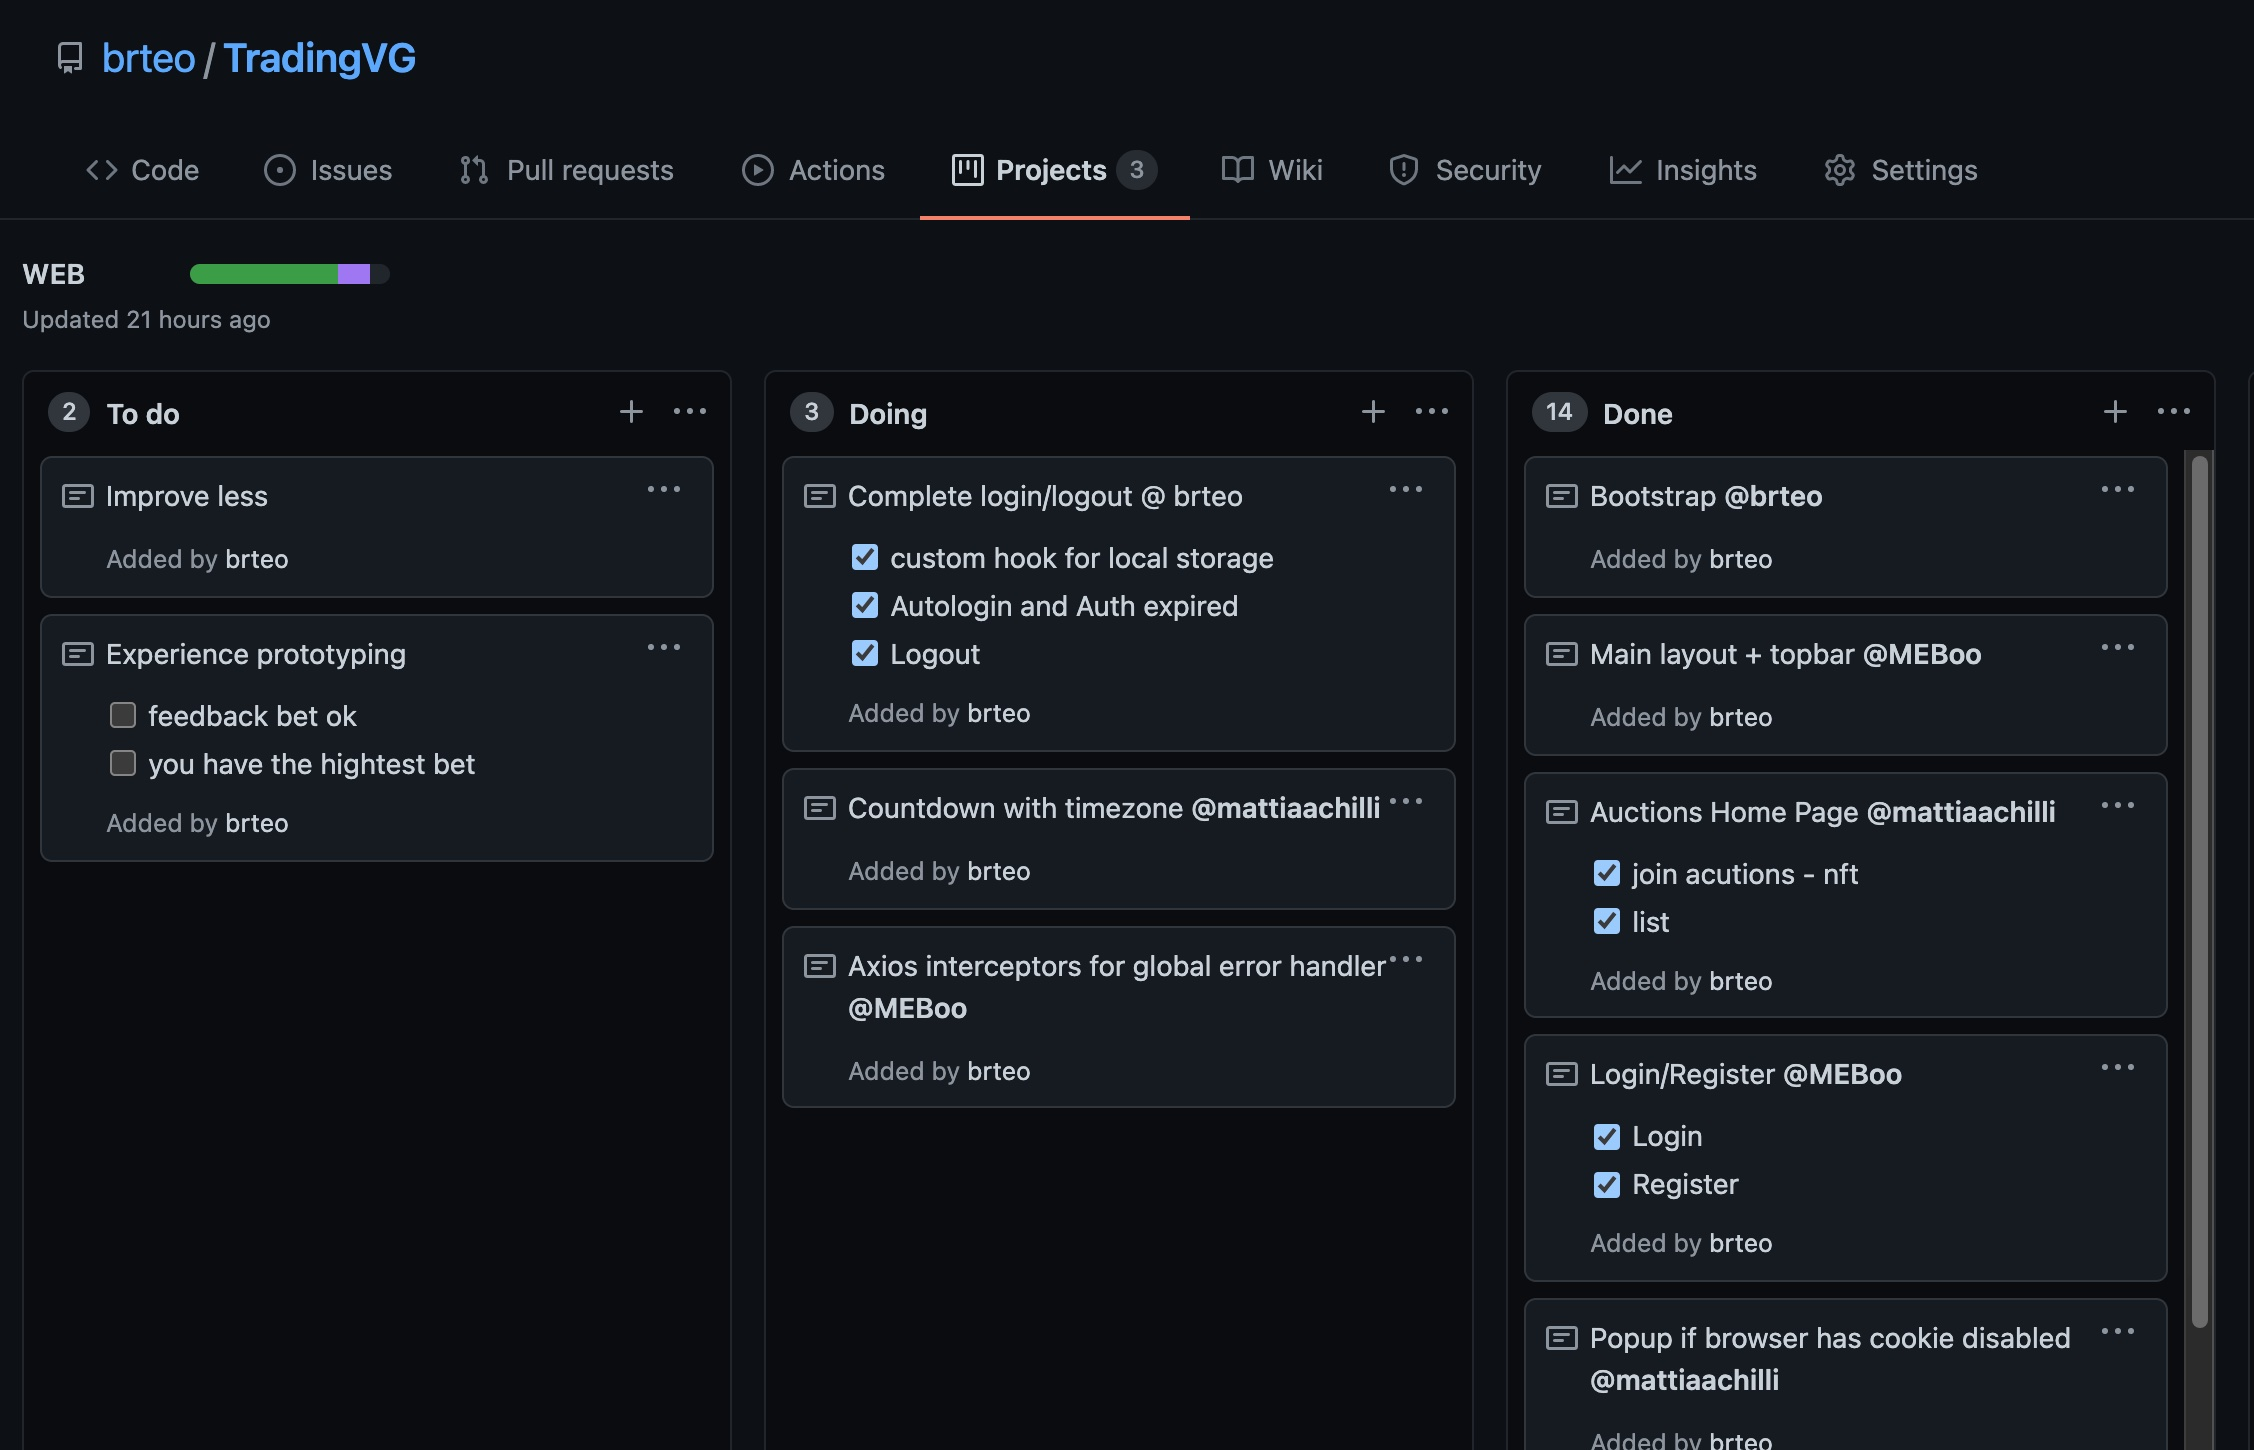
\includegraphics[width=\textwidth,keepaspectratio]{github-projects.jpg}
	\caption{GitHub Projects}
	\label{fig:github-projects}
\end{figure}

In questo modo siamo stati in grado di valutare progressivamente tutte le caratteristiche implementative ed accogliere i cambiamenti per tempo
dal momento che buona parte delle tecnologie si sono studiate durante la realizzazione del progetto.

Volendo utilizzare un approccio \textbf{User Centered Design}, durante l'intera fase di design e sviluppo,
ci si è focalizzati sui bisogni degli utenti al fine di creare un servizio che soddisfi gli utilizzatori.
In mancanza di utenti finali reali, durante le riunioni settimanali, 
il team valutava le funzionalità e l'interfaccia che stava prendendo forma immedesimandosi nelle \textbf{Personas} definite inizialmente [3.3.1].

Come strumento software a supporto si è deciso di utilizzare GitHub Projects all'interno del repository del progetto.

Infine abbiamo deciso fin dall'inizio di utilizzare il metodo \textbf{TDD} (Test Drive development) per quanto riguarda lo sviluppo della RestApi,
facendo in modo che tutti gli endpoint della RestApi siano oppurtunamente testati fin dall'inizio.

\subsection{Archittetura del sistema}
Dopo la definizione delle metodologie di sviluppo, ci siamo concentrati nella realizzazione dell'architettura del sistema.
Abbiamo immaginato che il portale web sia in futuro distribuito in moderne piattaforme cloud a microservizi.

\begin{figure}[H]
	\centering
	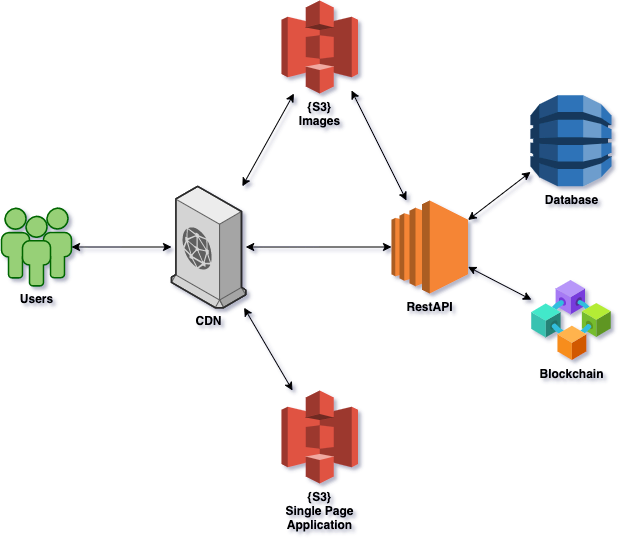
\includegraphics[width=0.7\textwidth,keepaspectratio]{architecture.png}
	\caption{Architettura del sistema}
	\label{fig:architecture}
\end{figure}

Gli utenti che navigheranno all'indirizzo web del portale accederanno alle risorse attraverso una \textbf{CDN} (Content Delivery Network),
una piattaforma di server altamente distribuita che aiuta a minimizzare il ritardo nel caricamento dei contenuti.

Il FrontEnd sarà una \textbf{SPA} (Single Page Application) ed in quanto tale potrà essere caricato su un Bucket \textbf{S3}. 
Le SPA sono applicazioni composte da una singola pagina non renderizzata lato server e
contenente tutto il codice necessario (HTML, JavaScript e CSS) recuperato in un singolo caricamento al prima accesso alla pagina.

Le altre risorse che compongono il portale saranno caricate dinamicamente secondo le esigenze attraverso chiamate al BackEnd dove sarà realizzata una RestApi 
che metterà a disposizione attraverso i suoi EndPoint le azioni di tipo CRUD (Create, Read, Update, Delete) 
utili a reperire e manipolare le informazioni salvate su \textbf{Database}.

La RestApi si dovrà interfacciare ad una \textbf{Blockchain} per la creazione e gestione degli NFT: un apposito Smart Contract dovrà essere progettato, implementato ed installato.

Infine le immagini saranno caricate su un'ulteriore Bucket \textbf{S3} per non appesantire la RestApi 
che deve restare sempre reattiva nello rispondere alle richieste degli utenti.

\subsection{Interfaccia utente}
Durante la fase di design abbiamo definito l'interfaccia utente 
e per tutta la durata del progetto l'abbiamo migliorata grazie ai meet settimanali dove ognuno di noi riportava i propri feedback,
immedesimandosi nei target users definiti inizialmente,
soprattutto nella fase finale quando il progetto prendeva sempre più forma e diventava un vero e proprio prototipo.

\subsubsection{Target Users}
Prima di pertire con lo sviluppo, quindi nelle primissime fasi del progetto, abbiamo cercato di identificare i terget users:
il portale sarà utilizzato dagli appassionati di arte digitale, principalmente suddivisi tra \textbf{collezionisti}, \textbf{creatori di opere} 
o semplici \textbf{speculatori} che vogliono cavalcare il momento con l'obiettivo di arricchirsi.

Immaginiamo un target per lo più composto da giovani, compreso tra i 15 ed i 35 anni, ma non escludiamo anche persone più adulte appassionate di tecnologia.
Con un target così giovane l'utilizzo di dispositivi mobile sarà sicuramente molto elevato,
di conseguenze un'interfaccia responsive è fondamentale per permettere agli utenti di avere una User Experience appagante ed intuitiva. 

Da questa riflessione iniziale sono state definite le seguenti \textbf{personas} 
utilizzate come riferimento per lo sviluippo dell'interfaccia e per il seed dei dati.

\bigbreak
\noindent
\textbf{Jhon}
\bigbreak
\noindent
Jhon ha 30 anni ed è un collezionista appassionato di arte e di tecnologia. 
Potremmo considerarlo un 'geek', abita ancora con i genitori e la sua camera è piena di fumetti, 
edizioni limitate di videogiochi e film, console del passato ed almeno un poster di Star Wars.

\underline{Scenario d'uso:}
Jhon scopre il nuovo portale per lo scambio di NFT, 
sa già che cosa sono in quanto appassionato di tecnologia 
e vuole accedere quotidianamente per verificare la presenza di nuove opere di suo gusto
così da partecipare alle aste per aggiudicarsele.

\begin{itemize}
	\item Entra sul portale
	\item Controlla la homepage dove immagina di trovare le ultime novità
	\item Non soddisfatto effettua una ricerca sul tema che più lo appassiona
	\item Trova l'NFT che sogna e decide subito di effettuare una puntata
	\item La prima volta gli verrà richeisto di registrarsi ma lui non ha problemi 
	\item Si registra 
	\item Effettua la puntata
\end{itemize}

\bigbreak
\noindent
\textbf{Tohoku}
\bigbreak
\noindent
Tohoku ha 16 anni e le piace disegnare, lo fa di continuo, anche a scuola durante le lezioni che la annoiano.
La ragazza non sa se farà l'università, non gli piace nessun lavoro, gli piace solo disegnare
ma in questo periodo storico sa già che sarà difficile renderlo un lavoro.

\underline{Scenario d'uso:}
Tra gli amici di Tohoku gira voce di questi nuovi NFT, dei token digitali che scambiarsi opere digitali,
ci sono persone che con i CryptoKitties hanno fatto un sacco di soldi! 
Tohoku sul treno di ritorno da scuola, tramite il suo smartphone cerca di informarsi e scopre il portale.

\begin{itemize}
	\item Entra sul portale
	\item Naviga le pagine per farsi un'idea
	\item Vuole creare subito il suo NFT con l'ultimo disegno fatto a scuola anche se non sa niente della tecnologia
	\item Le verrà richiesta la registrazione
	\item Crea il suo primo NFT
\end{itemize}

\bigbreak
\noindent
\textbf{Mario}
\bigbreak
\noindent
Mario ha 52 anni è un fotografo da una vita, ha viaggiato il mondo e lavora per qualche redazione importante.
La fotografia è la sua passione ma a è al servizio di altri che lo pagano per fare reportage.

\underline{Scenario d'uso:}
Mario sa utilizzare il computer ed i social, visto anche il lavoro che svolge, ed un giorno legge degli NFT sul sole24ore.
Ha subito una illuminazione: da quando è arrivato internet non ha mai saputo come proteggere le proprie foto pubblicate online, 
sul suo sito fatto dal nipote o sui social che detengono tutti i diritti, e finalmente pensa che questa nuova tecnologia può proteggere il suo copyright.
Effettua subito delle ricerche sul suo iMac da 27 pollici e finisce sul portale.

\begin{itemize}
	\item Entra sul portale
	\item Naviga le pagine per farsi un'idea
	\item Legge tutta la privacy e termini e condizioni d'uso del sito
	\item Si fida e vuole creare il suo NFT con la foto che più gli piace dell'ultimo anno ma che non aveva ancora pubblicato
	\item Gli verrà richiesta la registrazione
	\item Crea il suo primo NFT
\end{itemize}

\bigbreak
\noindent
\textbf{dark02}
\bigbreak
\noindent
Dark02 è il suo nickname, non sappiamo il suo nome e la sua età, sappiamo solo che è giovane ed un appasisonato di tecnologia,
naviga tutti i forum e cerca sempre il modo di cavalcare qualche moda per fare soldi, 
ne ha fatti tanti con i Bitcoin e CryptoKitties.

\underline{Scenario d'uso:}
Dark02 viene a conoscenza del nuovo portale in poco tempo, ha le sue fonti e subito si interessa è tra i primi a registrarsi.
Viene spesso sul portale, vuole comprare partecipando alle aste con l'augurio che prendano valore, ma allo stesso tempo vuole creare i suoi NFT, 
riciclando illustrazioni fatte dalla ex ragazza.

\begin{itemize}
	\item Entra sul portale
	\item Accede perchè già registrato
	\item Controlla la homepage
	\item Trova subito quello che vuole ed entra nel dettaglio
	\item Partecipa all'asta
	\item Cerca altri NFT dello stesso tipo
	\item Partecipa anche a questi
	\item Infine crea il suo NFT, na ha giò creati tanti.
\end{itemize}

\clearpage

\subsubsection{Mockups/Prototipo}
Inizialmente abbiamo immaginato il layout del sito attraverso degli sketch su carta.

Ci siamo concentrati a realizzare un web design incentrato sui contenuti e responsivo: diversi dispositivi, stessa esperienza.

\begin{figure}[H]
	\centering
	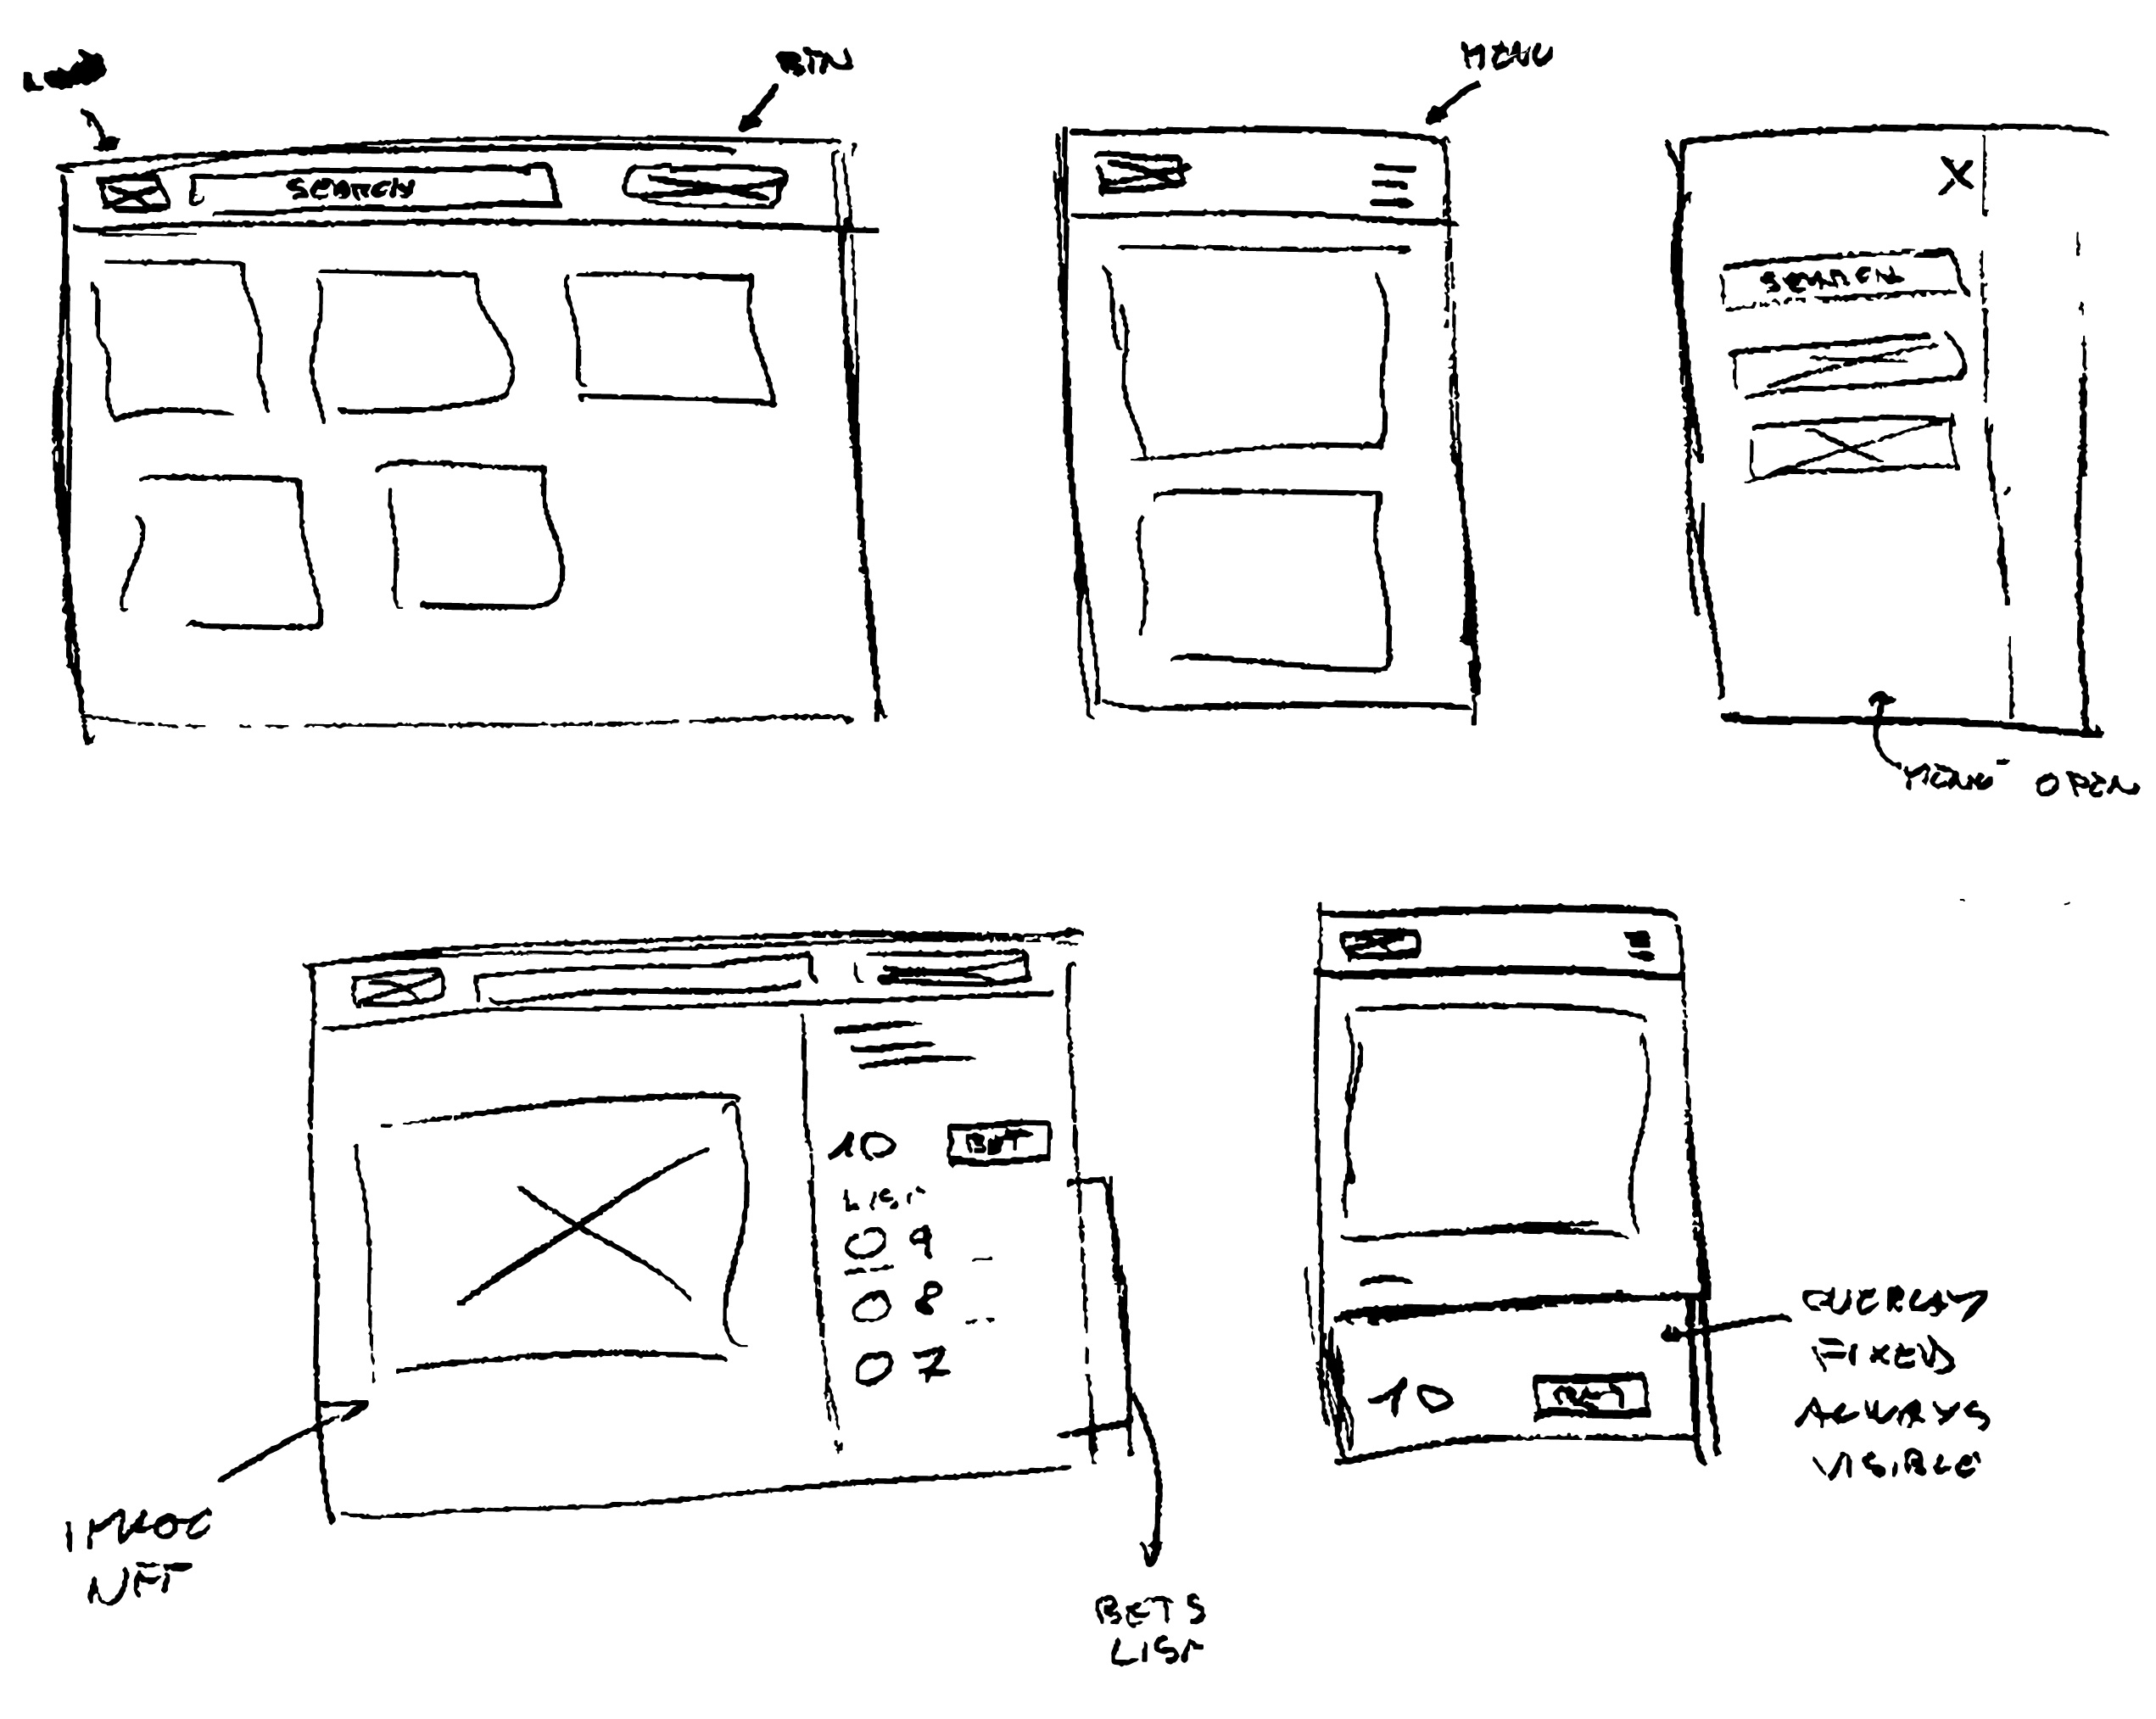
\includegraphics[width=\textwidth,keepaspectratio]{sketch.jpg}
	\caption{Sketch iniziale}
	\label{fig:sketch}
\end{figure}

Partendo da questi sketch, la UI ha preso forma durante lo sviluppo ed è stata progressivamente migliorata.

Per quanto riguarda l'estetica abbiamo pensato di incentrarla sul colore giallo oro, 
per far percepire il contesto di "prezioso" che governa i contenuti.

Scegliendo il colore giallo abbiamo subito capito che lo sfondo del sito sarebbe dovuto essere scuro 
altrimenti ci sarebbero stati problemi di contrasto non rendendo semplice la lettura e comprensione dell'interfaccia, 
soprattutto a persone con problemi di vista.
\bigbreak
\noindent
Caratteristiche dell'interfaccia decise fin da subito:
\begin{itemize}
	\item Il colore giallo predominante sul sito e legato al brand sarebbe dovuto essere utilizzato per ogni componente interattivo: pulsanti e link.
	\item Intestazione del sito sempre visibile con ricerca, pulsante per la creazione di NFT, accesso  e possibilità di cambiare lingua.
	Su dispositivi smartphone, in mancanza di spazio, questi componenti saranno accessibili in un classico menu "mobile" 
	che gli utenti sono abituati a trovare sul web ed accessibili tramite la classica "hamburger icon"
	\item Sfruttare tutta la grandezza del monitor, anche su dispositivi di grandi dimensioni con risoluzione FullHD
	\item Nella pagina dell'asta, l'interfaccia per eseguire la puntata deve essere sempre ben visibile, 
	l'utente non deve far fatica a trovarla o perderla scorrendo la pagina
	\item Accesso e registrazione in "Google style", descritto più aventi.
\end{itemize}

\clearpage

\bigbreak
\noindent
\textbf{Desktop 1280x800px}

\begin{figure}[H]
	\centering
	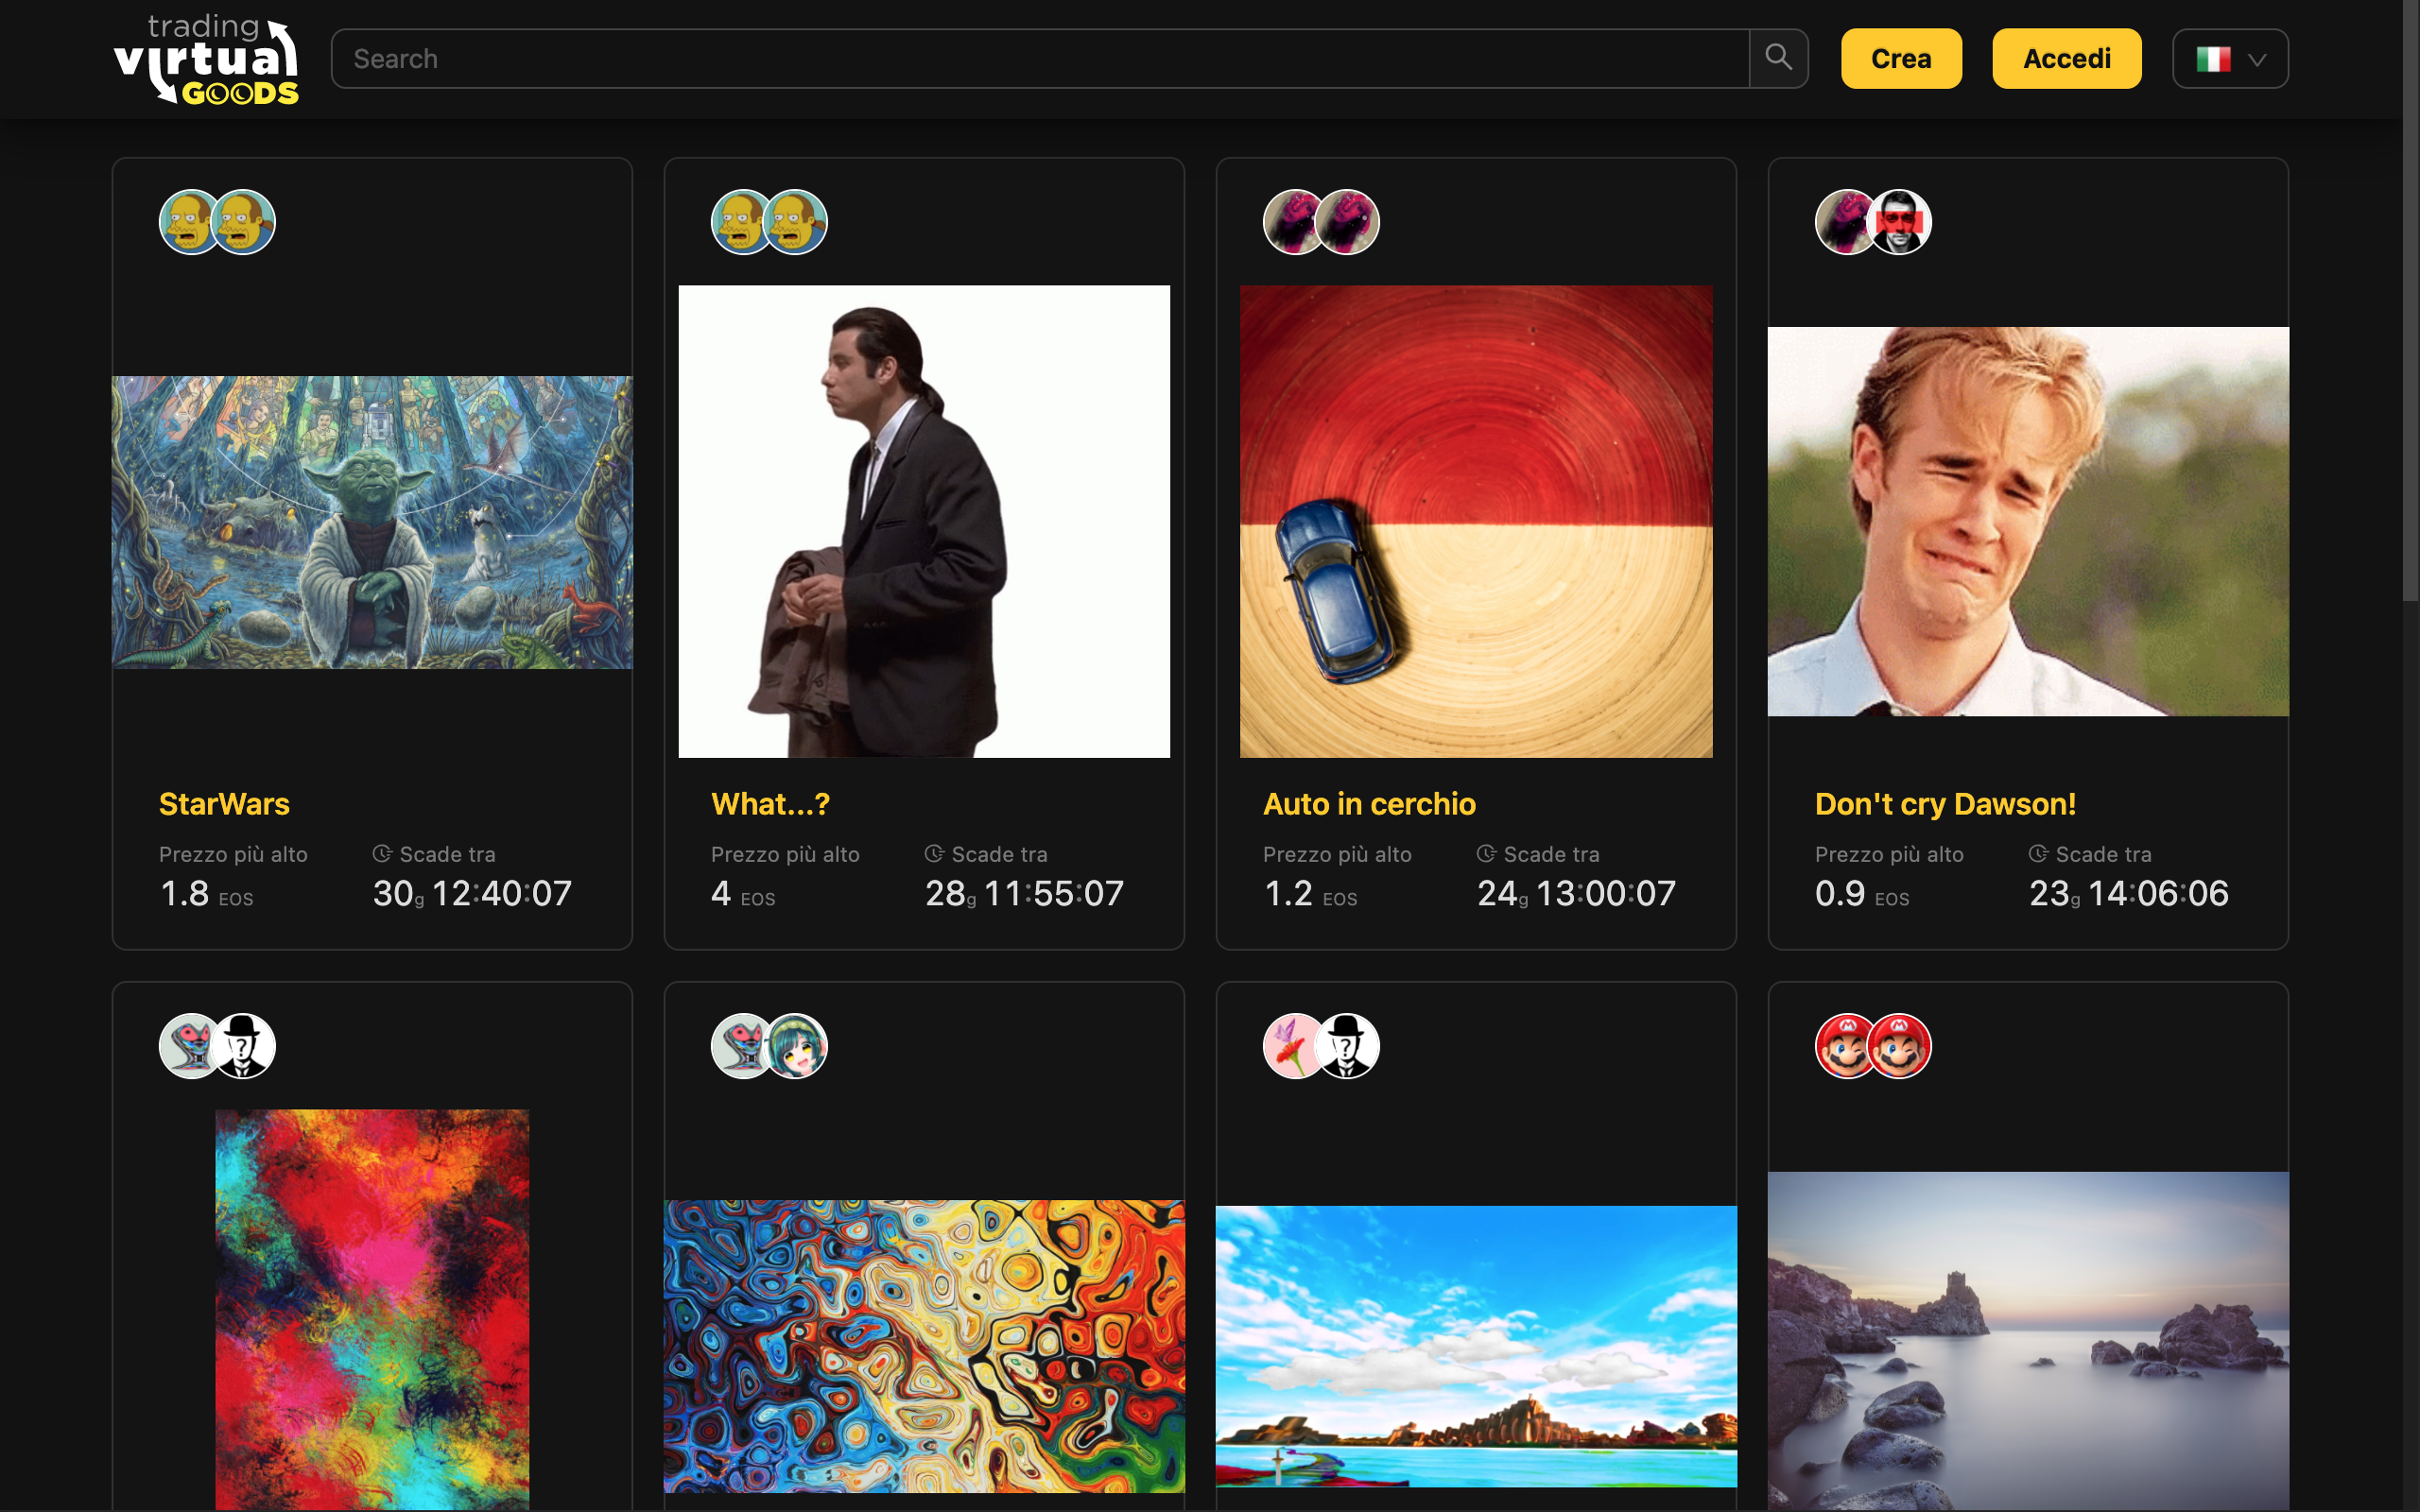
\includegraphics[width=0.85\textwidth,keepaspectratio]{p-desktop-home.jpg}
	\caption{Homepage}
	\label{fig:pDesktopHome}
\end{figure}
\begin{figure}[H]
	\centering
	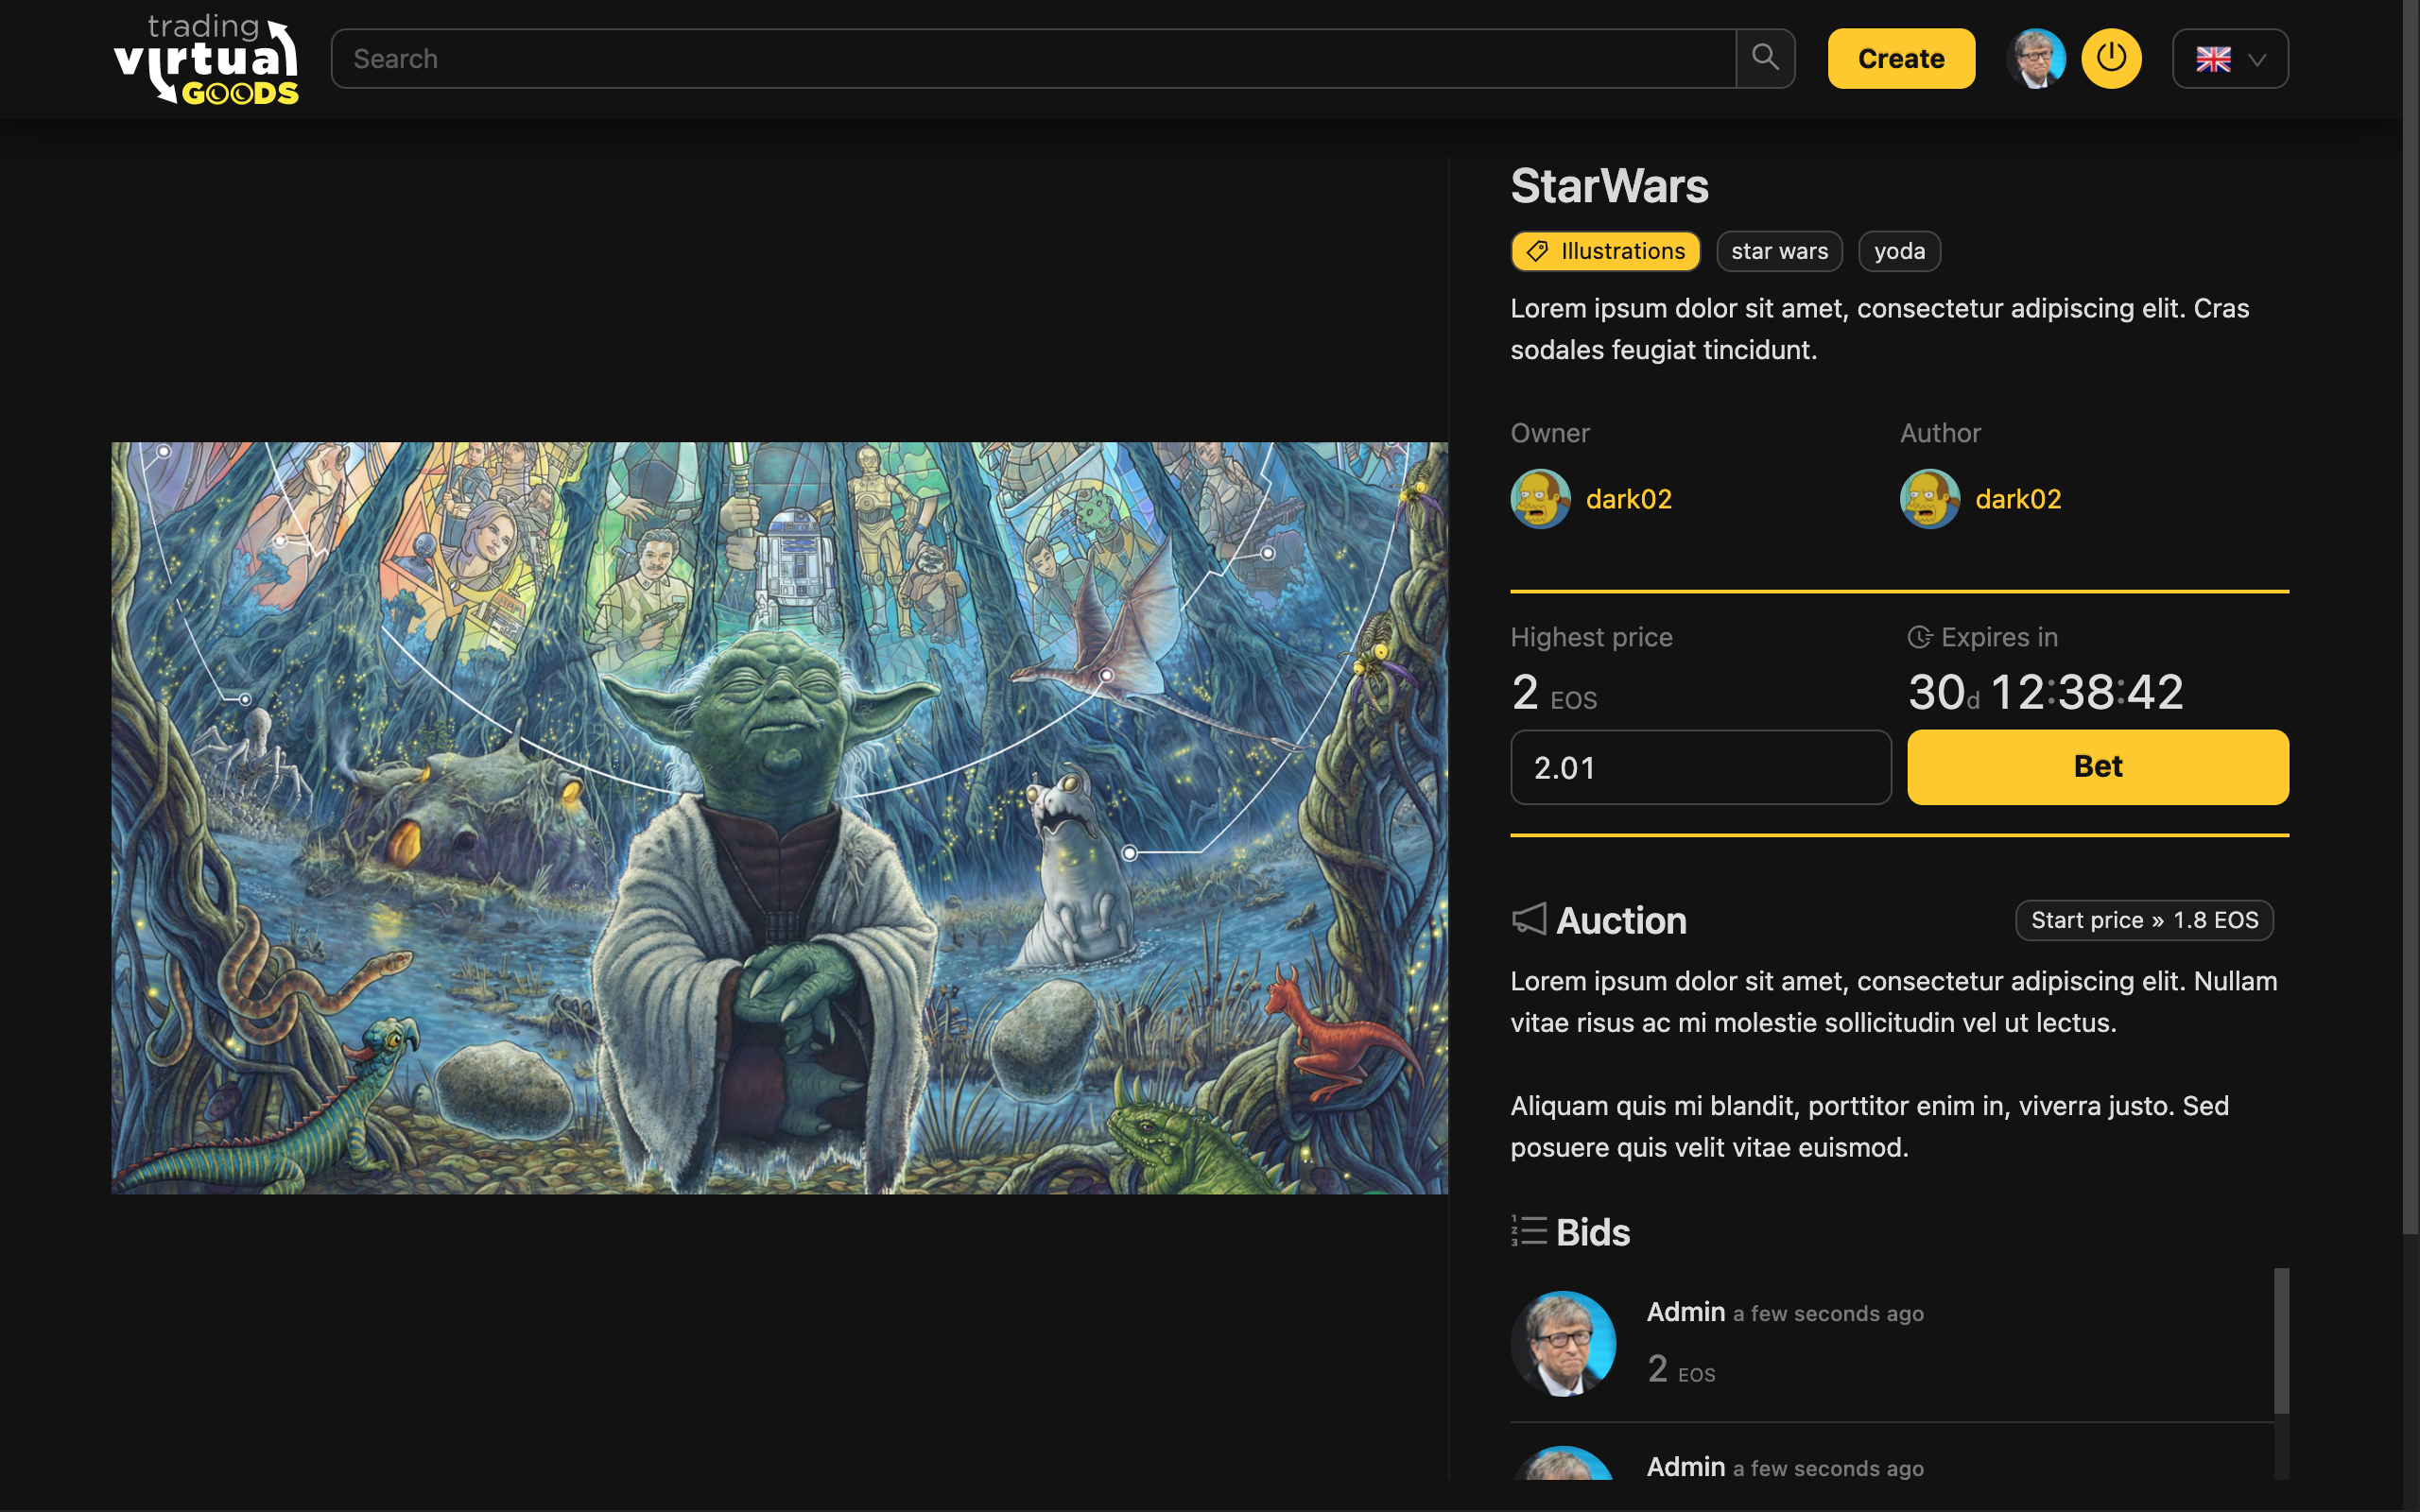
\includegraphics[width=0.85\textwidth,keepaspectratio]{p-desktop-auction.jpg}
	\caption{Pagina asta}
	\label{fig:pDesktopAuction}
\end{figure}
\begin{figure}[H]
	\centering
	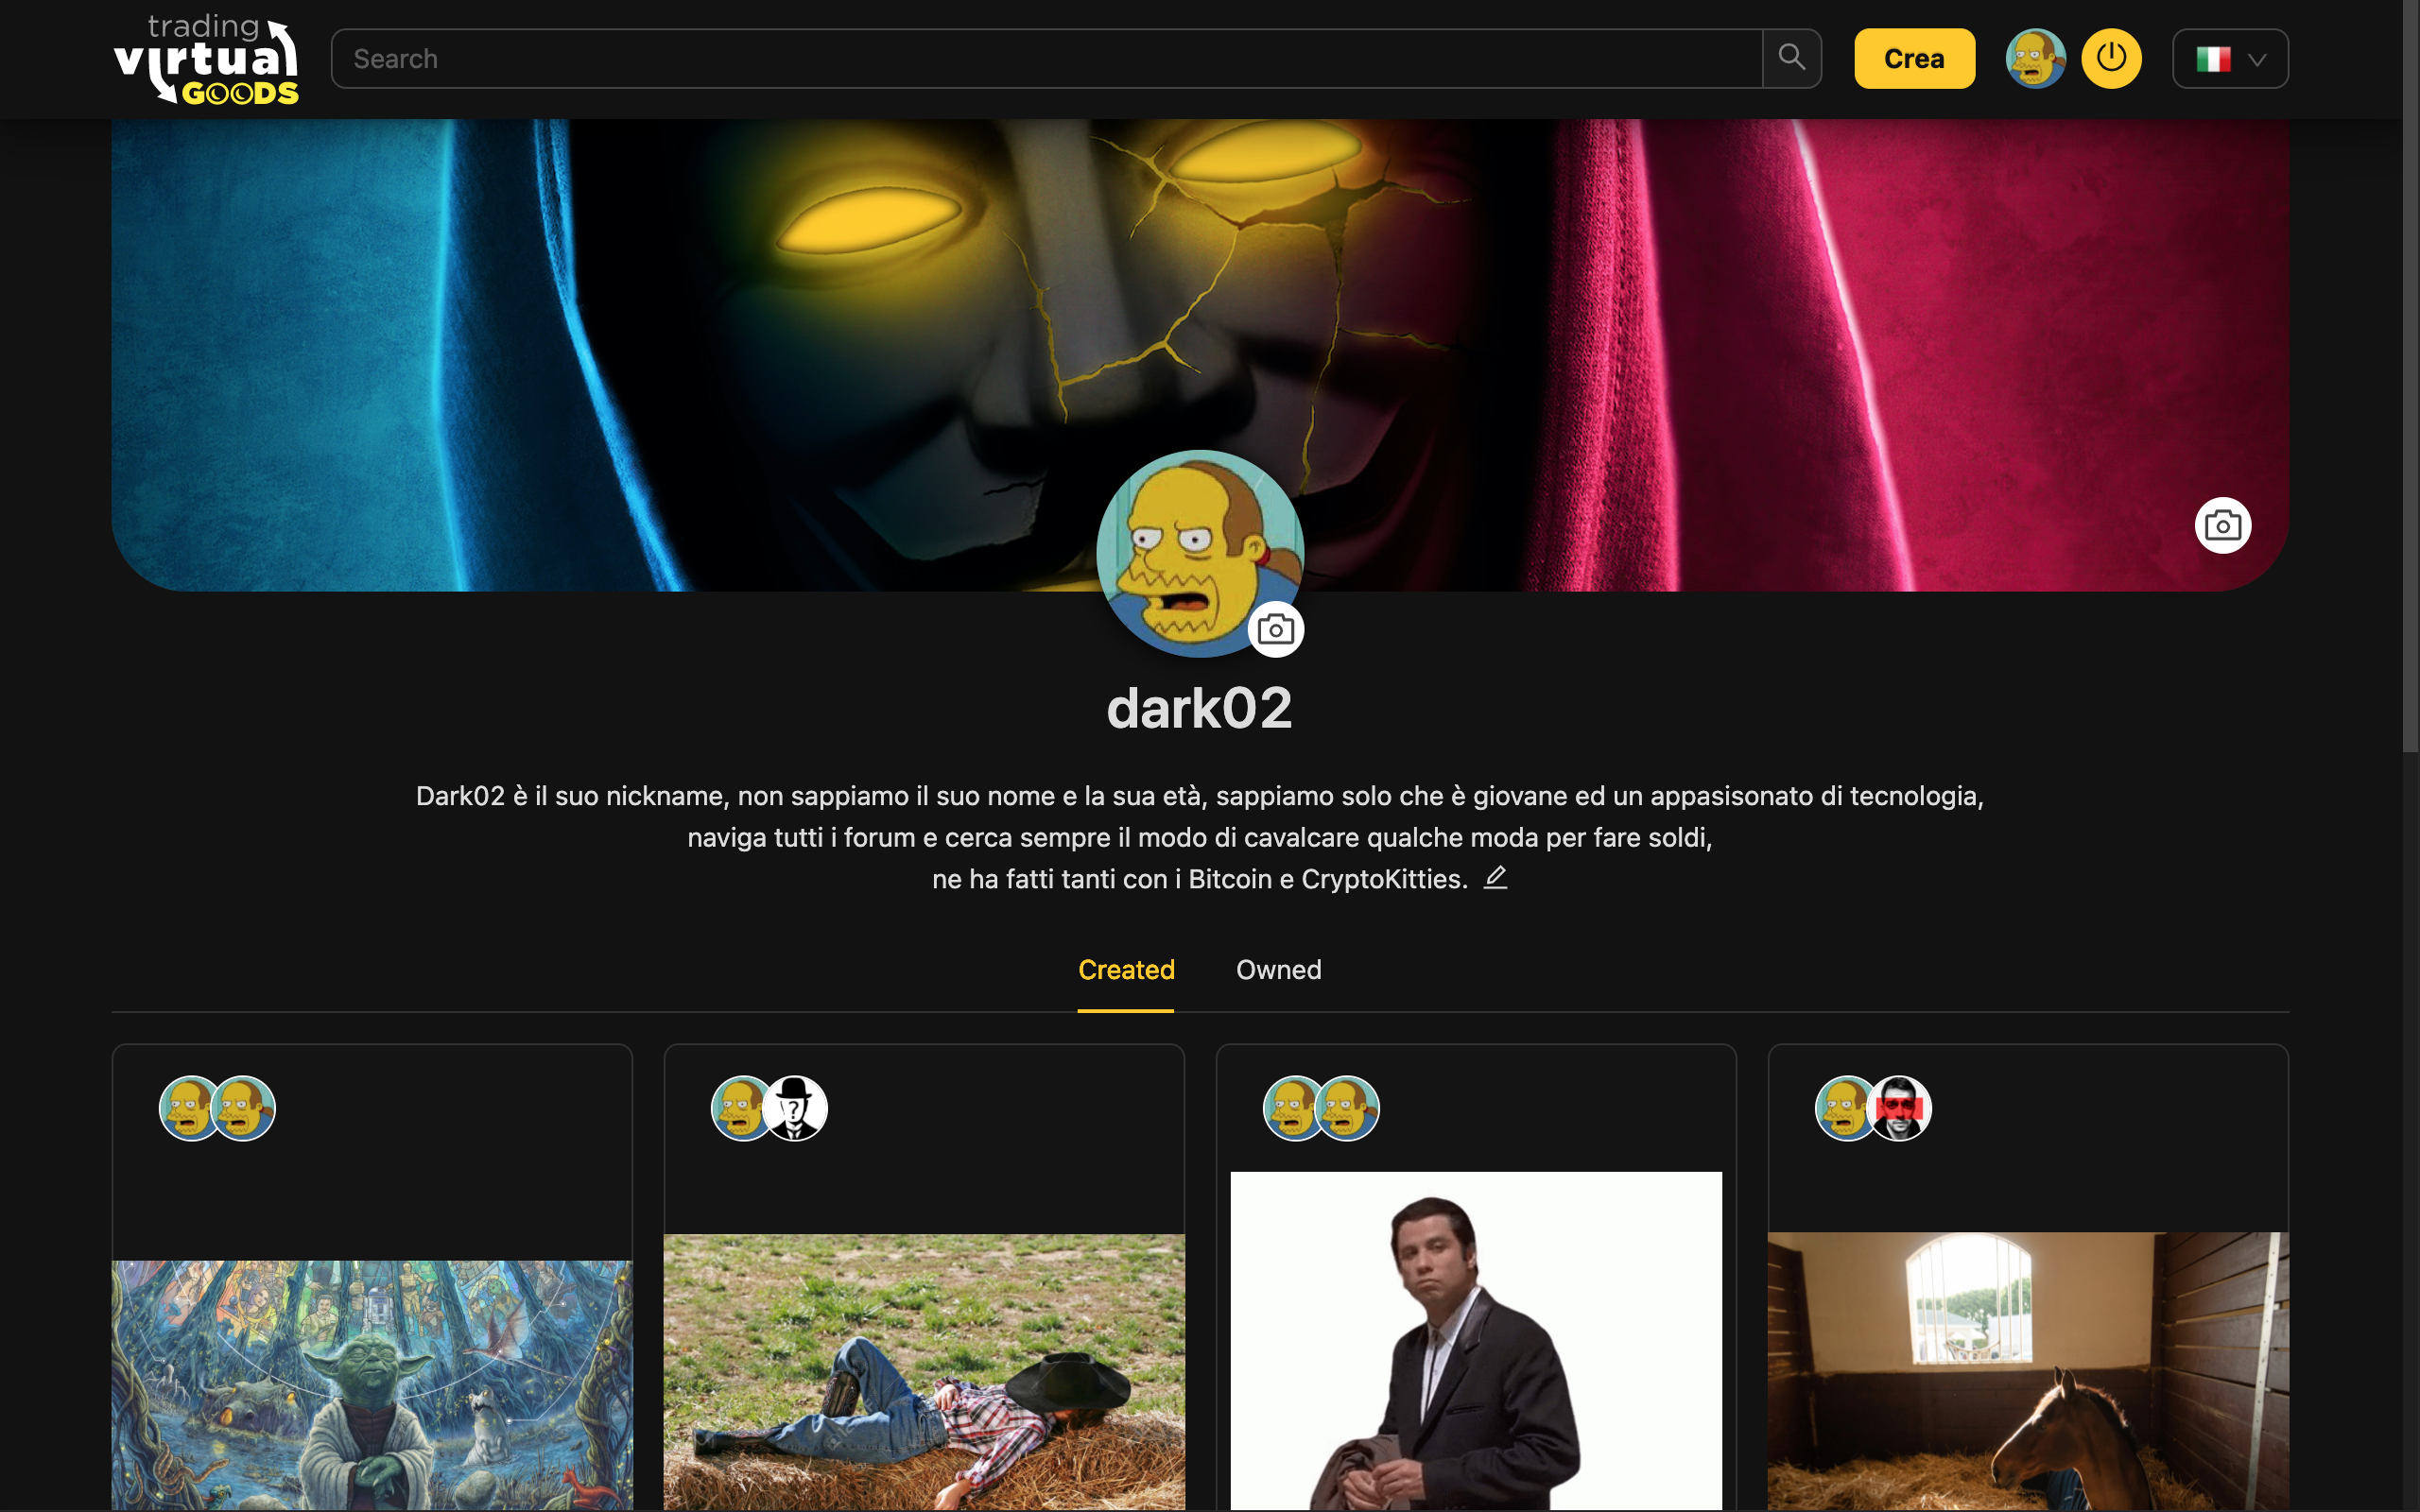
\includegraphics[width=0.85\textwidth,keepaspectratio]{p-desktop-profile.jpg}
	\caption{Pagina profilo}
	\label{fig:pDesktopProfile}
\end{figure}
\begin{figure}[H]
	\centering
	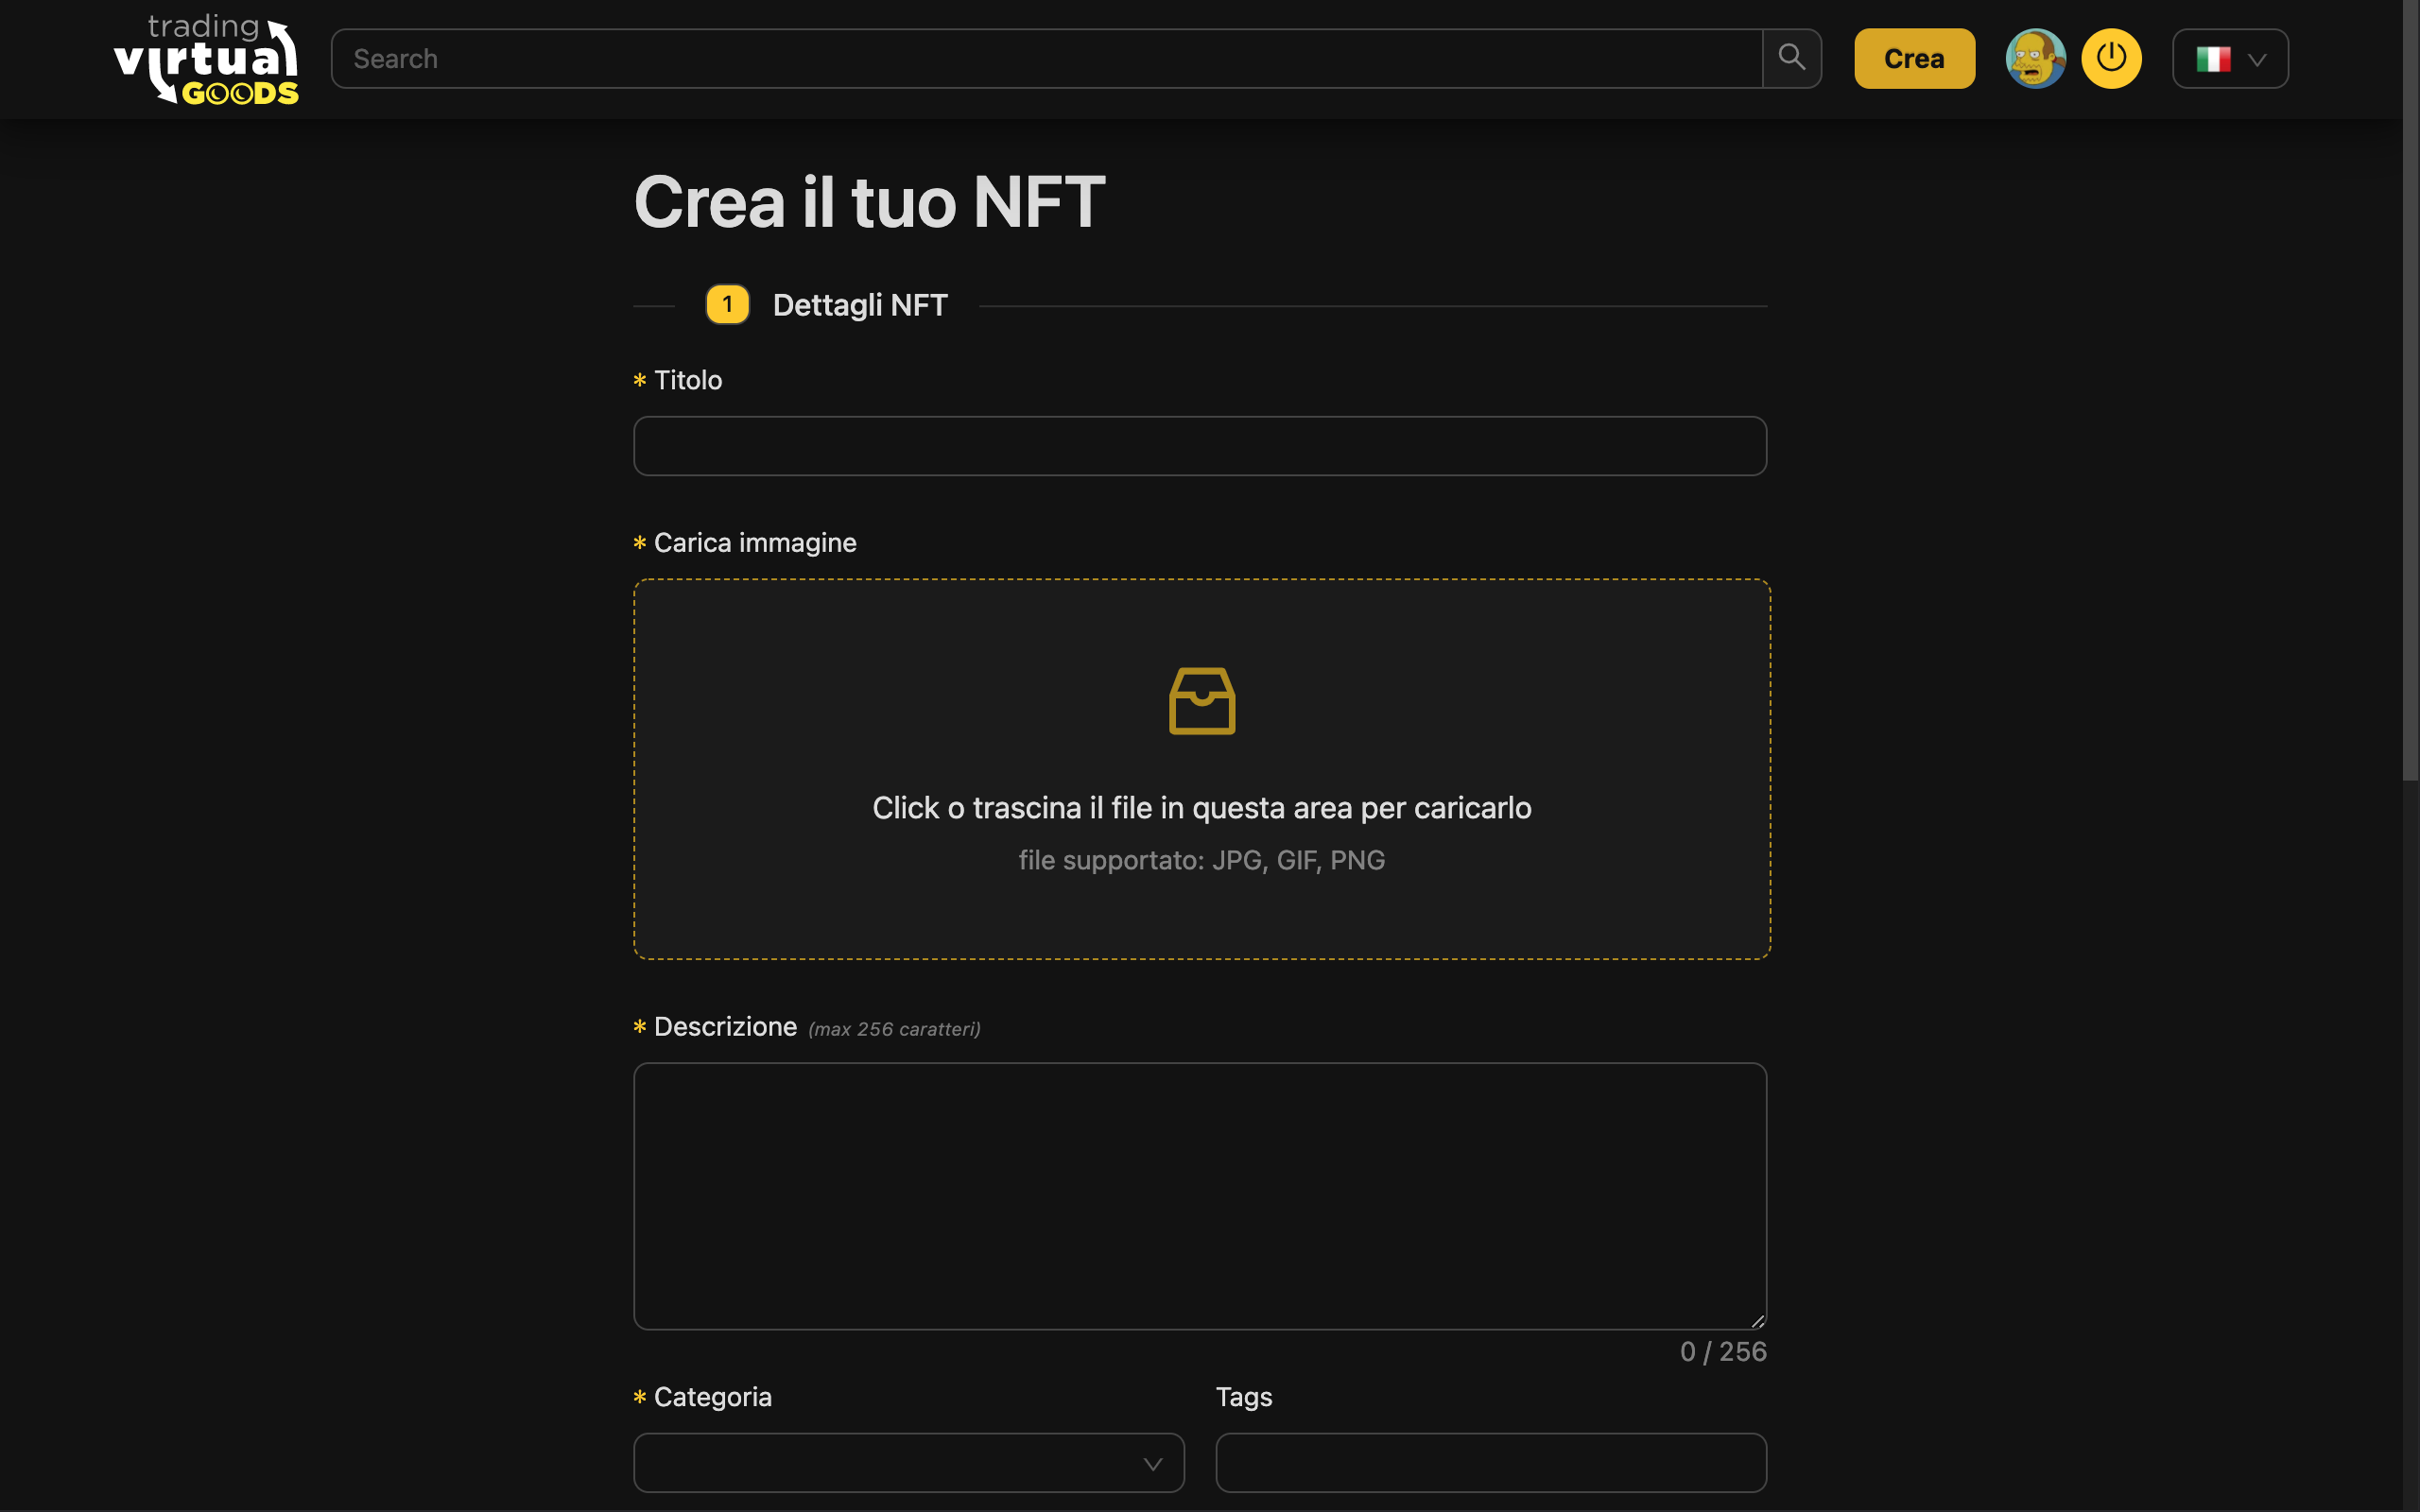
\includegraphics[width=0.85\textwidth,keepaspectratio]{p-desktop-create.jpg}
	\caption{Pagina creazione NFT}
	\label{fig:pDesktopCreate}
\end{figure}

\clearpage

\bigbreak
\noindent
\textbf{Smartphone portrait 375x667px}

\begin{figure}[H]
	\centering
	\begin{minipage}[b]{0.48\textwidth}
		\centering
		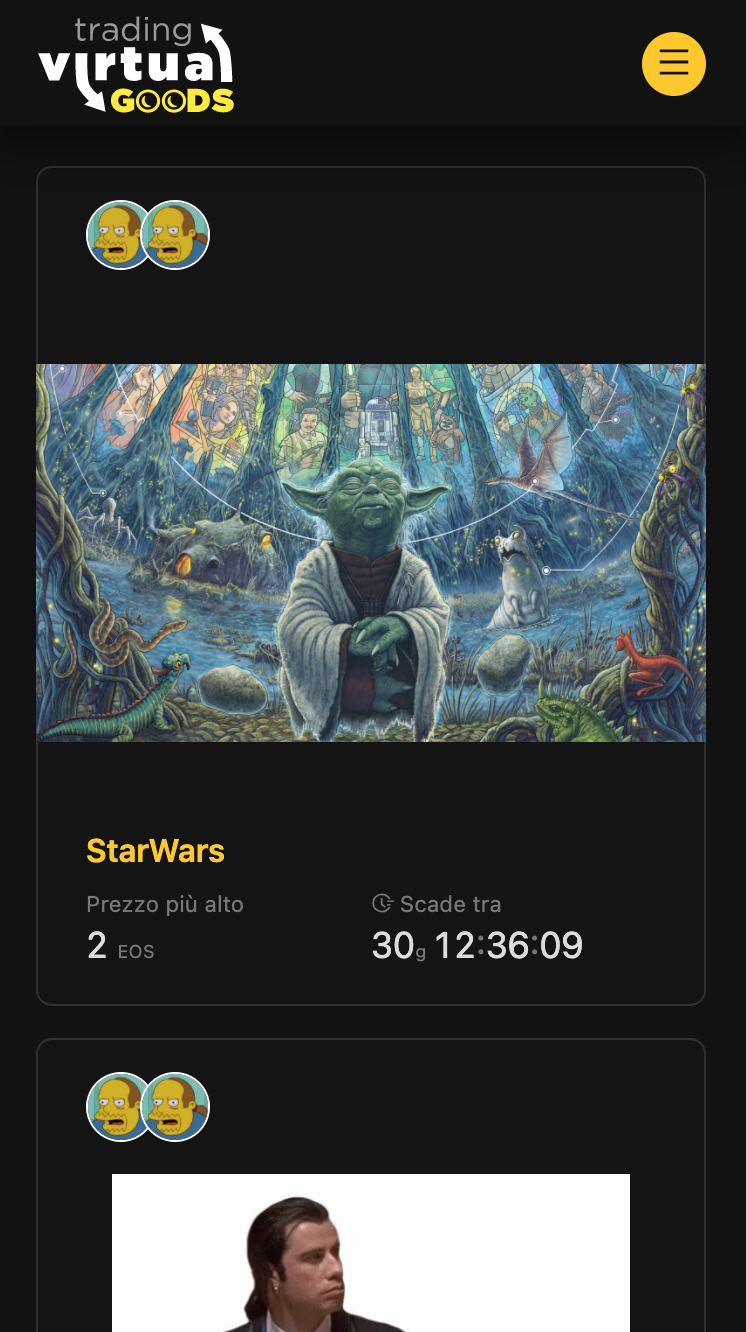
\includegraphics[width=\linewidth,keepaspectratio]{p-mobile-home.jpg}
		\caption{Homepage}
		\label{fig:pMobileHome}
	\end{minipage}
	\begin{minipage}[b]{0.48\textwidth}
		\centering
		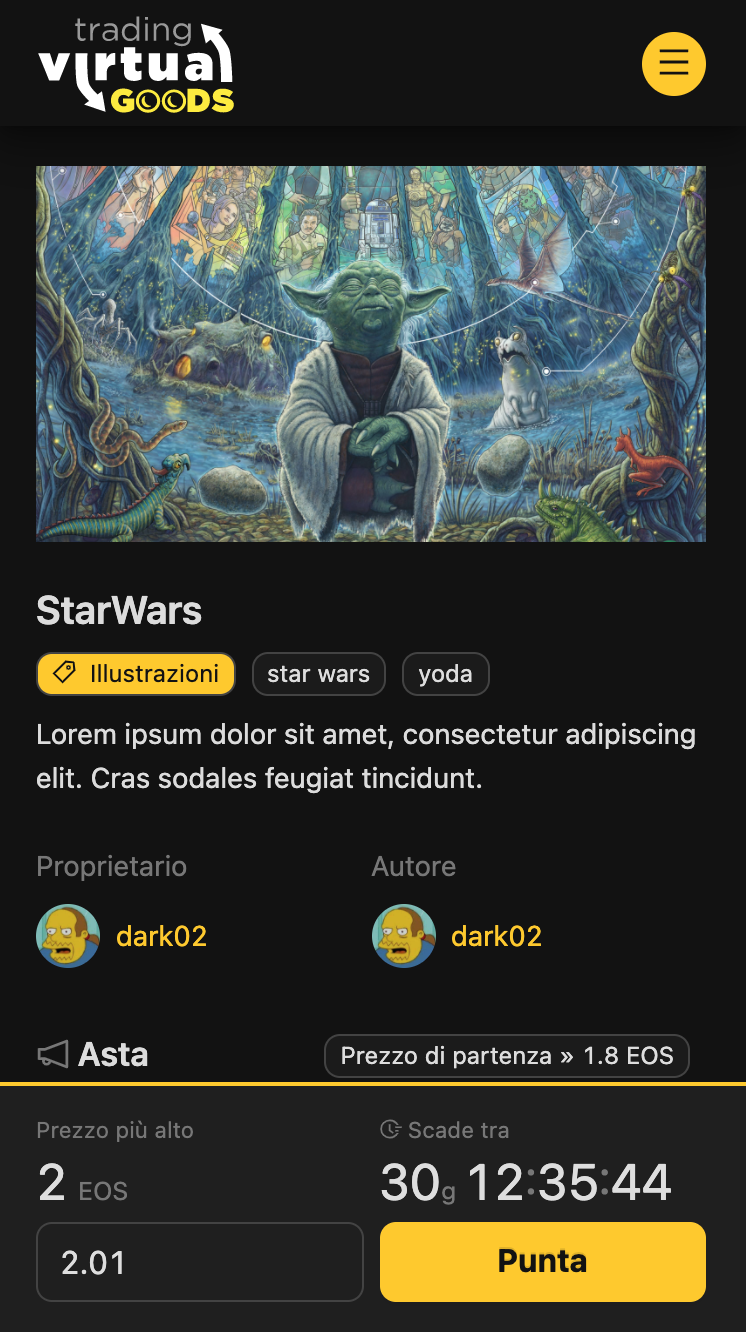
\includegraphics[width=\linewidth,keepaspectratio]{p-mobile-auction.jpg}
		\caption{Pagina asta}
		\label{fig:pMobileAuction}
	\end{minipage}	
\end{figure}

\begin{figure}[H]
	\centering
	\begin{minipage}[b]{0.48\textwidth}
		\centering
		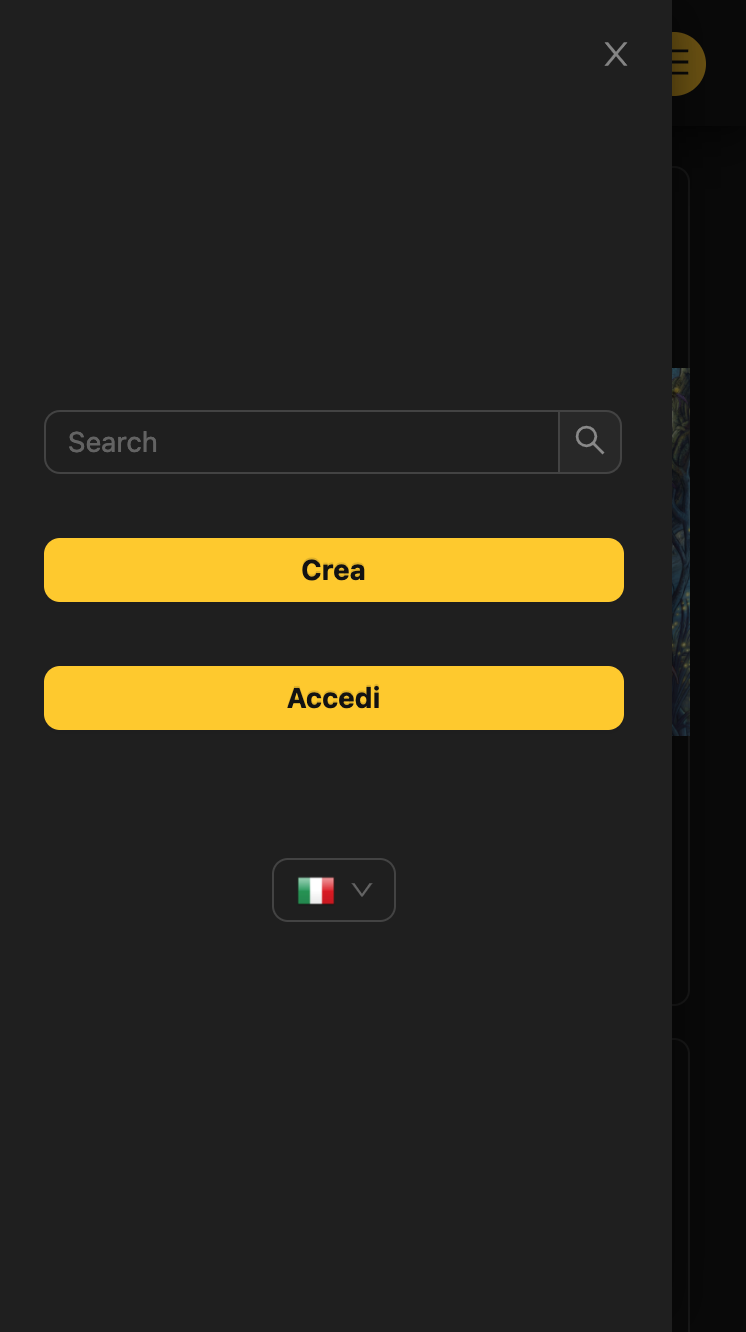
\includegraphics[width=\linewidth,keepaspectratio]{p-mobile-home-menu.jpg}
		\caption{Mobile menù aperto}
		\label{fig:pMobileHomeMenu}
	\end{minipage}
	\begin{minipage}[b]{0.48\textwidth}
		\centering
		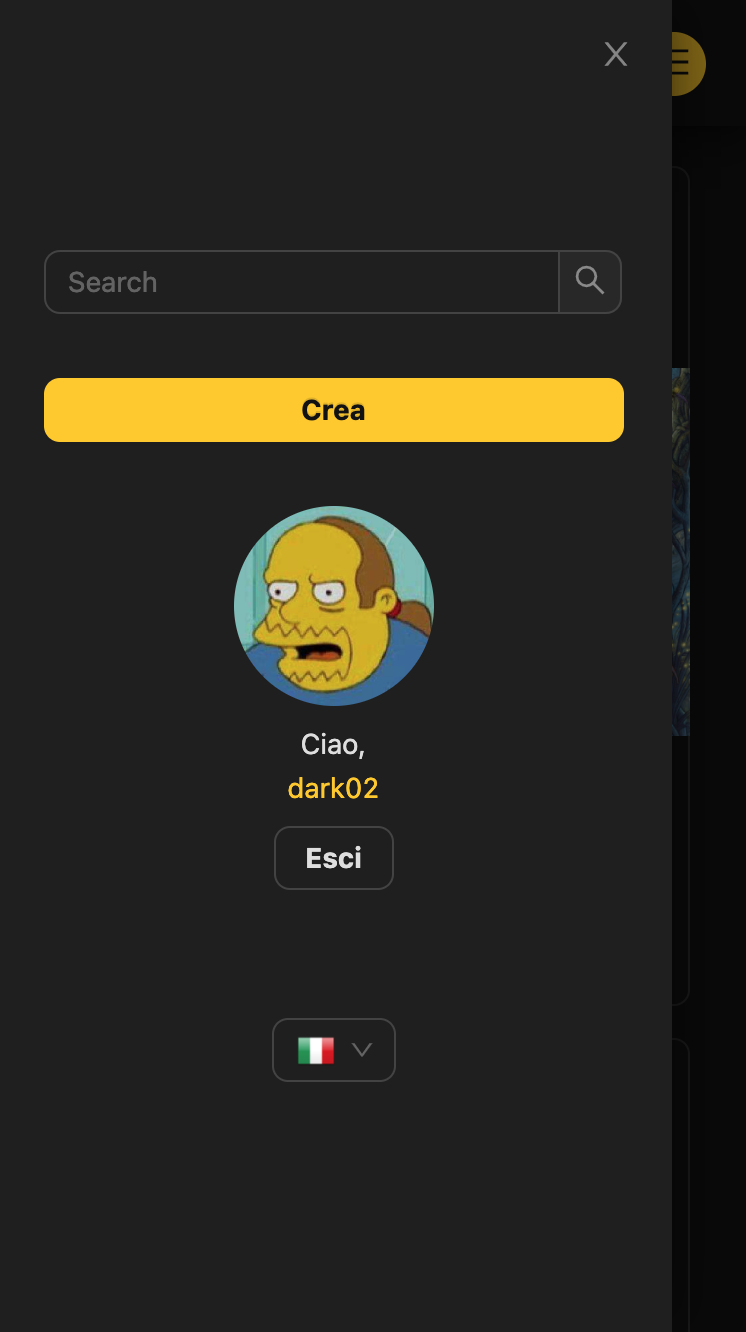
\includegraphics[width=\linewidth,keepaspectratio]{p-mobile-home-menu2.jpg}
		\caption{Mobile menù loggato}
		\label{fig:pMobileHomeMenu2}
	\end{minipage}	
\end{figure}

\begin{figure}[H]
	\centering
	\begin{minipage}[b]{0.48\textwidth}
		\centering
		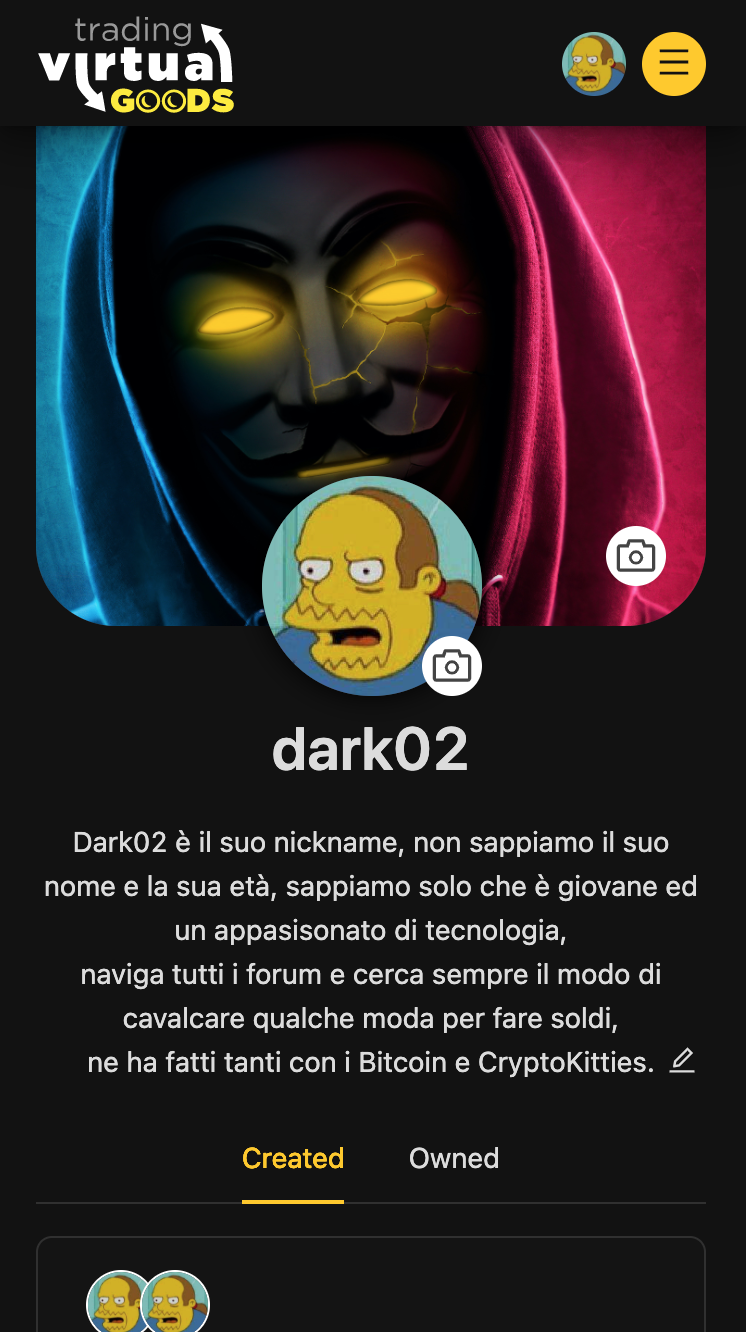
\includegraphics[width=\linewidth,keepaspectratio]{p-mobile-profile.jpg}
		\caption{Pagina profilo}
		\label{fig:pMobileProfile}
	\end{minipage}	
	\begin{minipage}[b]{0.48\textwidth}
		\centering
		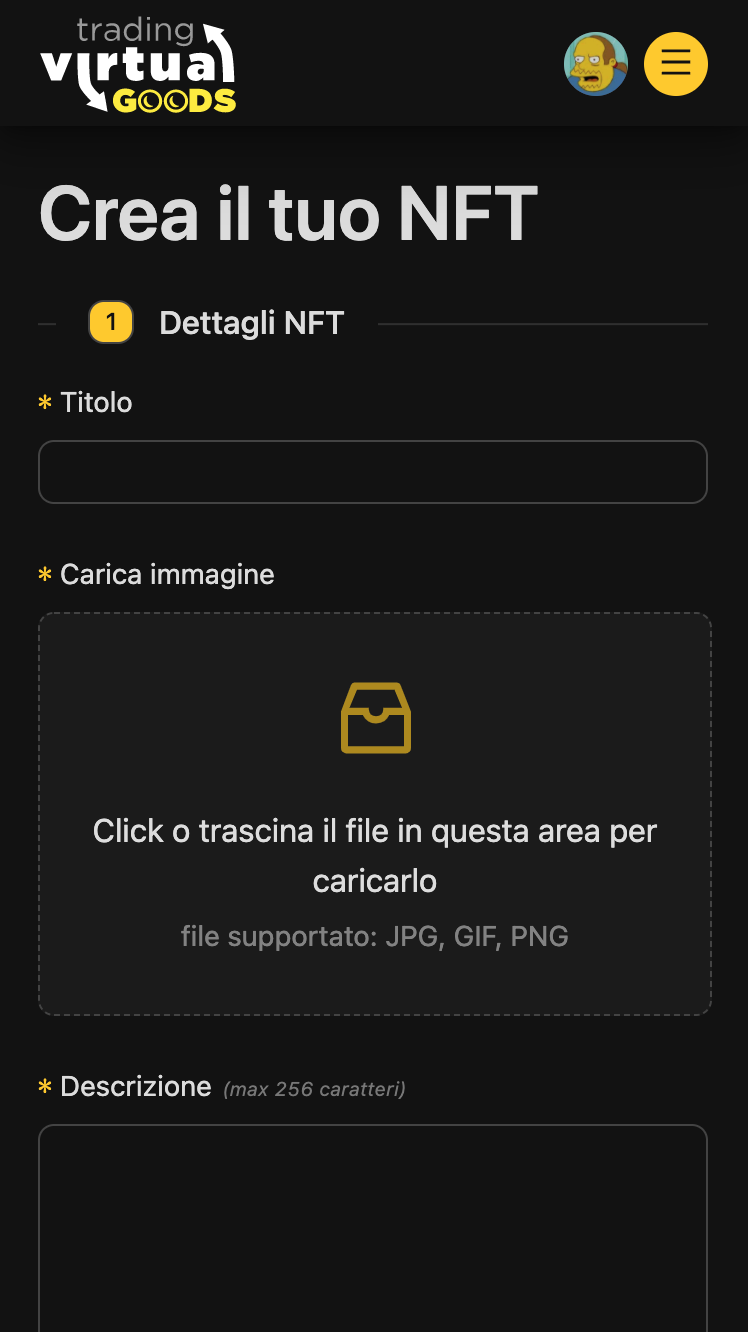
\includegraphics[width=\linewidth,keepaspectratio]{p-mobile-create.jpg}
		\caption{Pagina creazione NFT}
		\label{fig:pMobileCreate}
	\end{minipage}
\end{figure}

\clearpage

\bigbreak
\noindent
\textbf{Tablet portrait 786x1024px}

\begin{figure}[H]
	\centering
	\begin{minipage}[b]{0.48\textwidth}
		\centering
		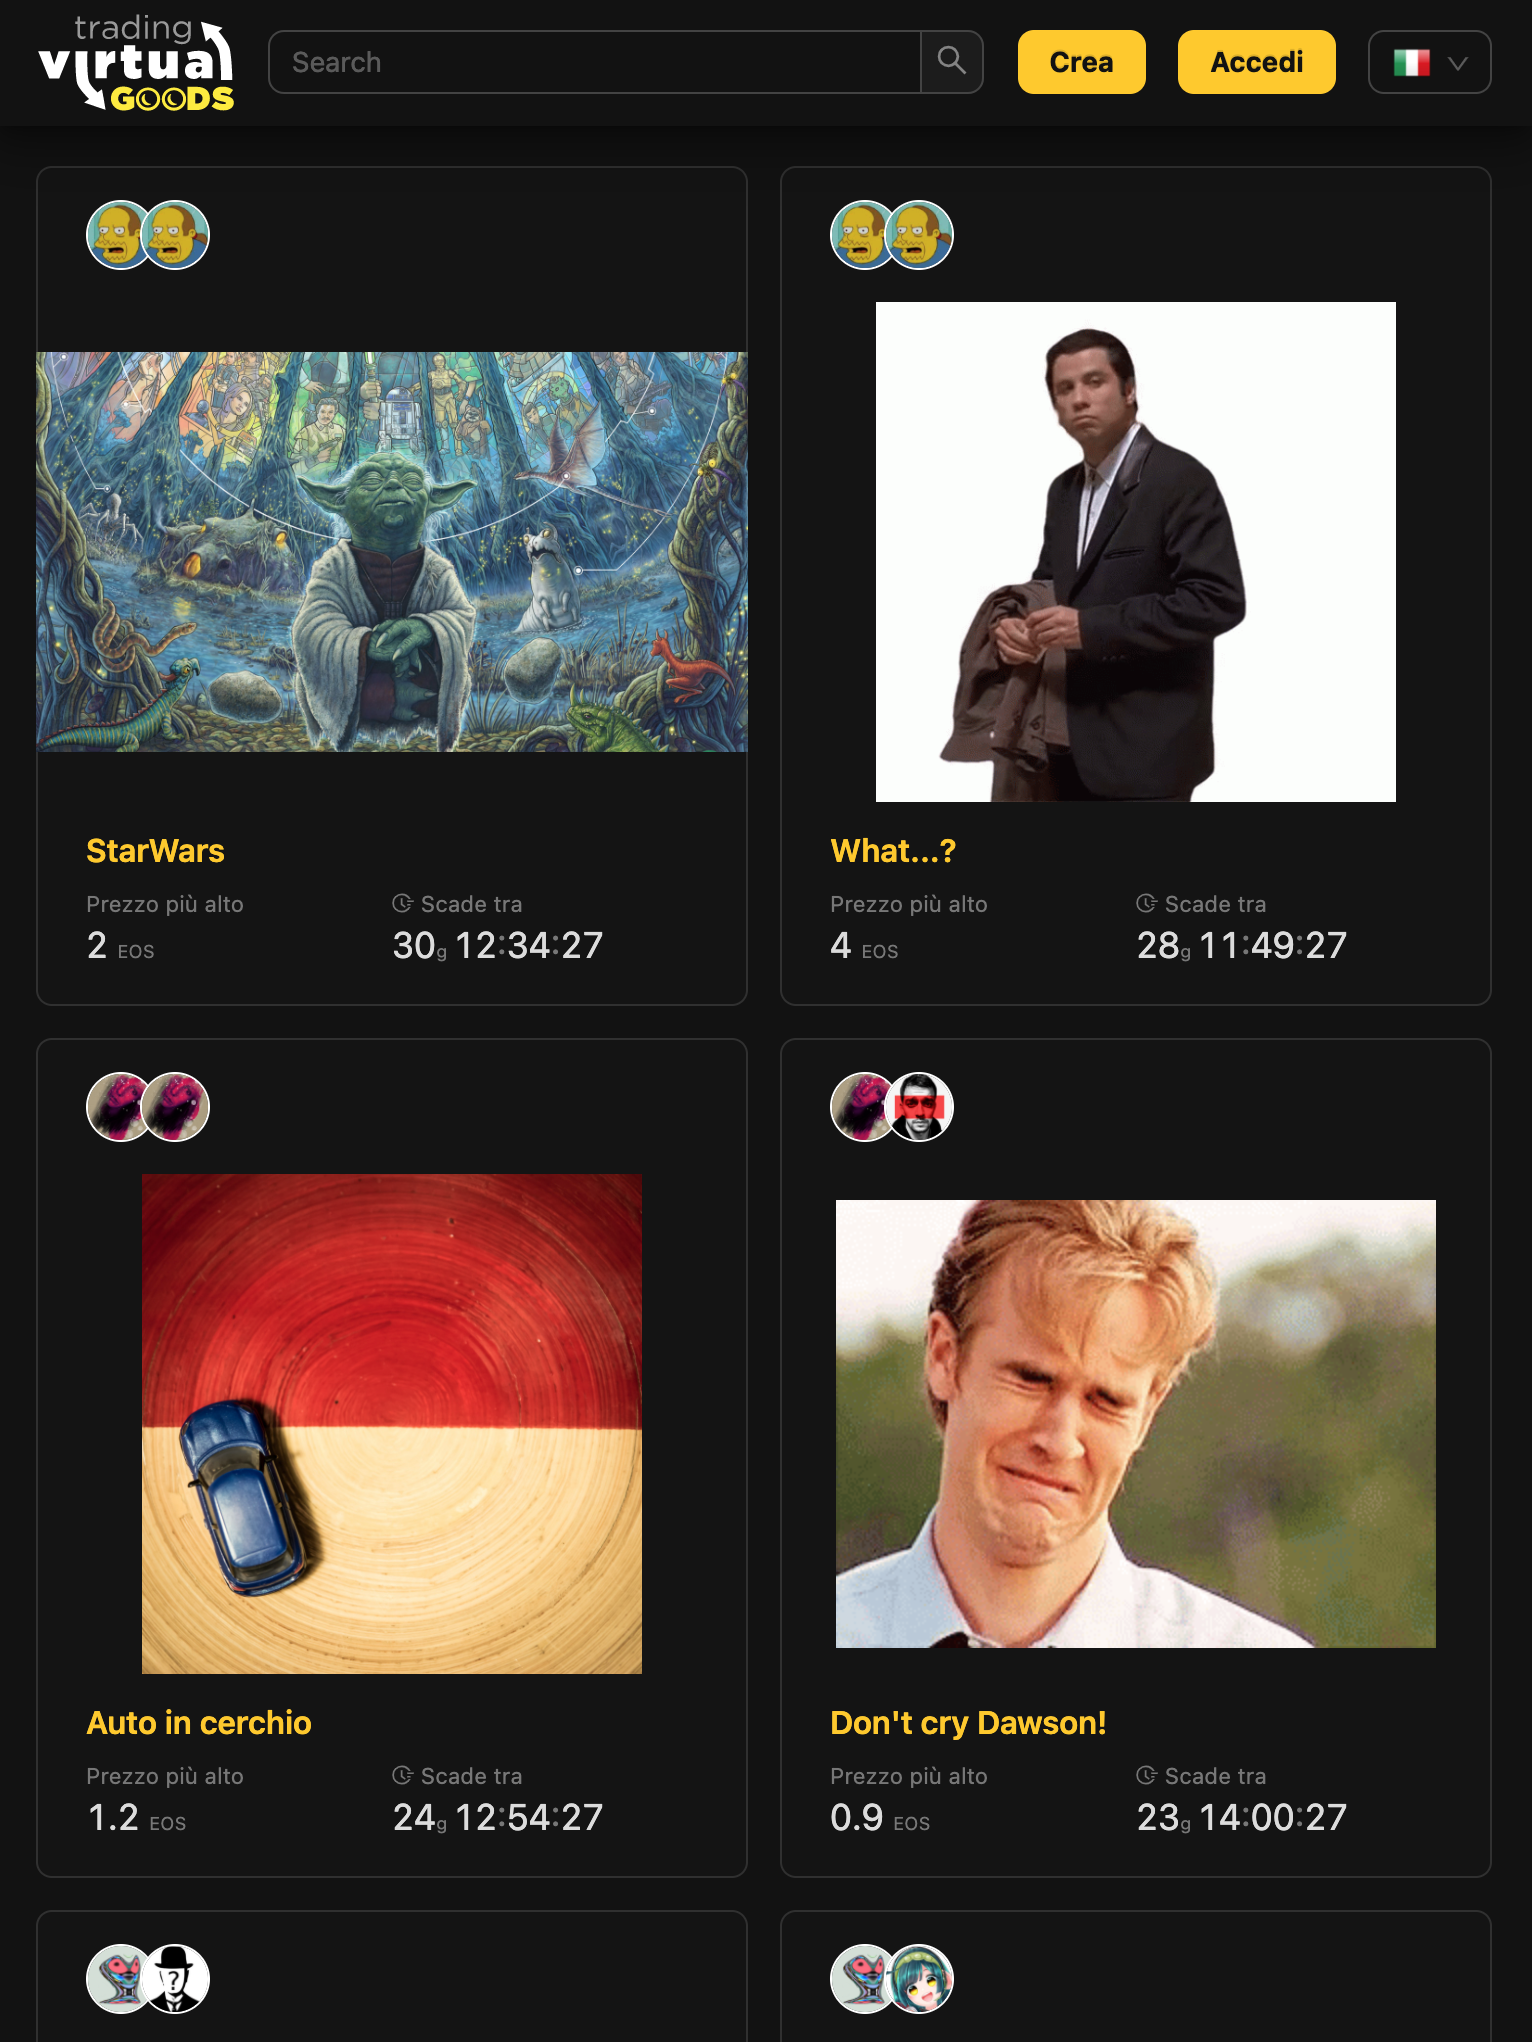
\includegraphics[width=\linewidth,keepaspectratio]{p-tablet-home.jpg}
		\caption{Homepage}
		\label{fig:pTabletHome}
	\end{minipage}	
	\begin{minipage}[b]{0.48\textwidth}
		\centering
		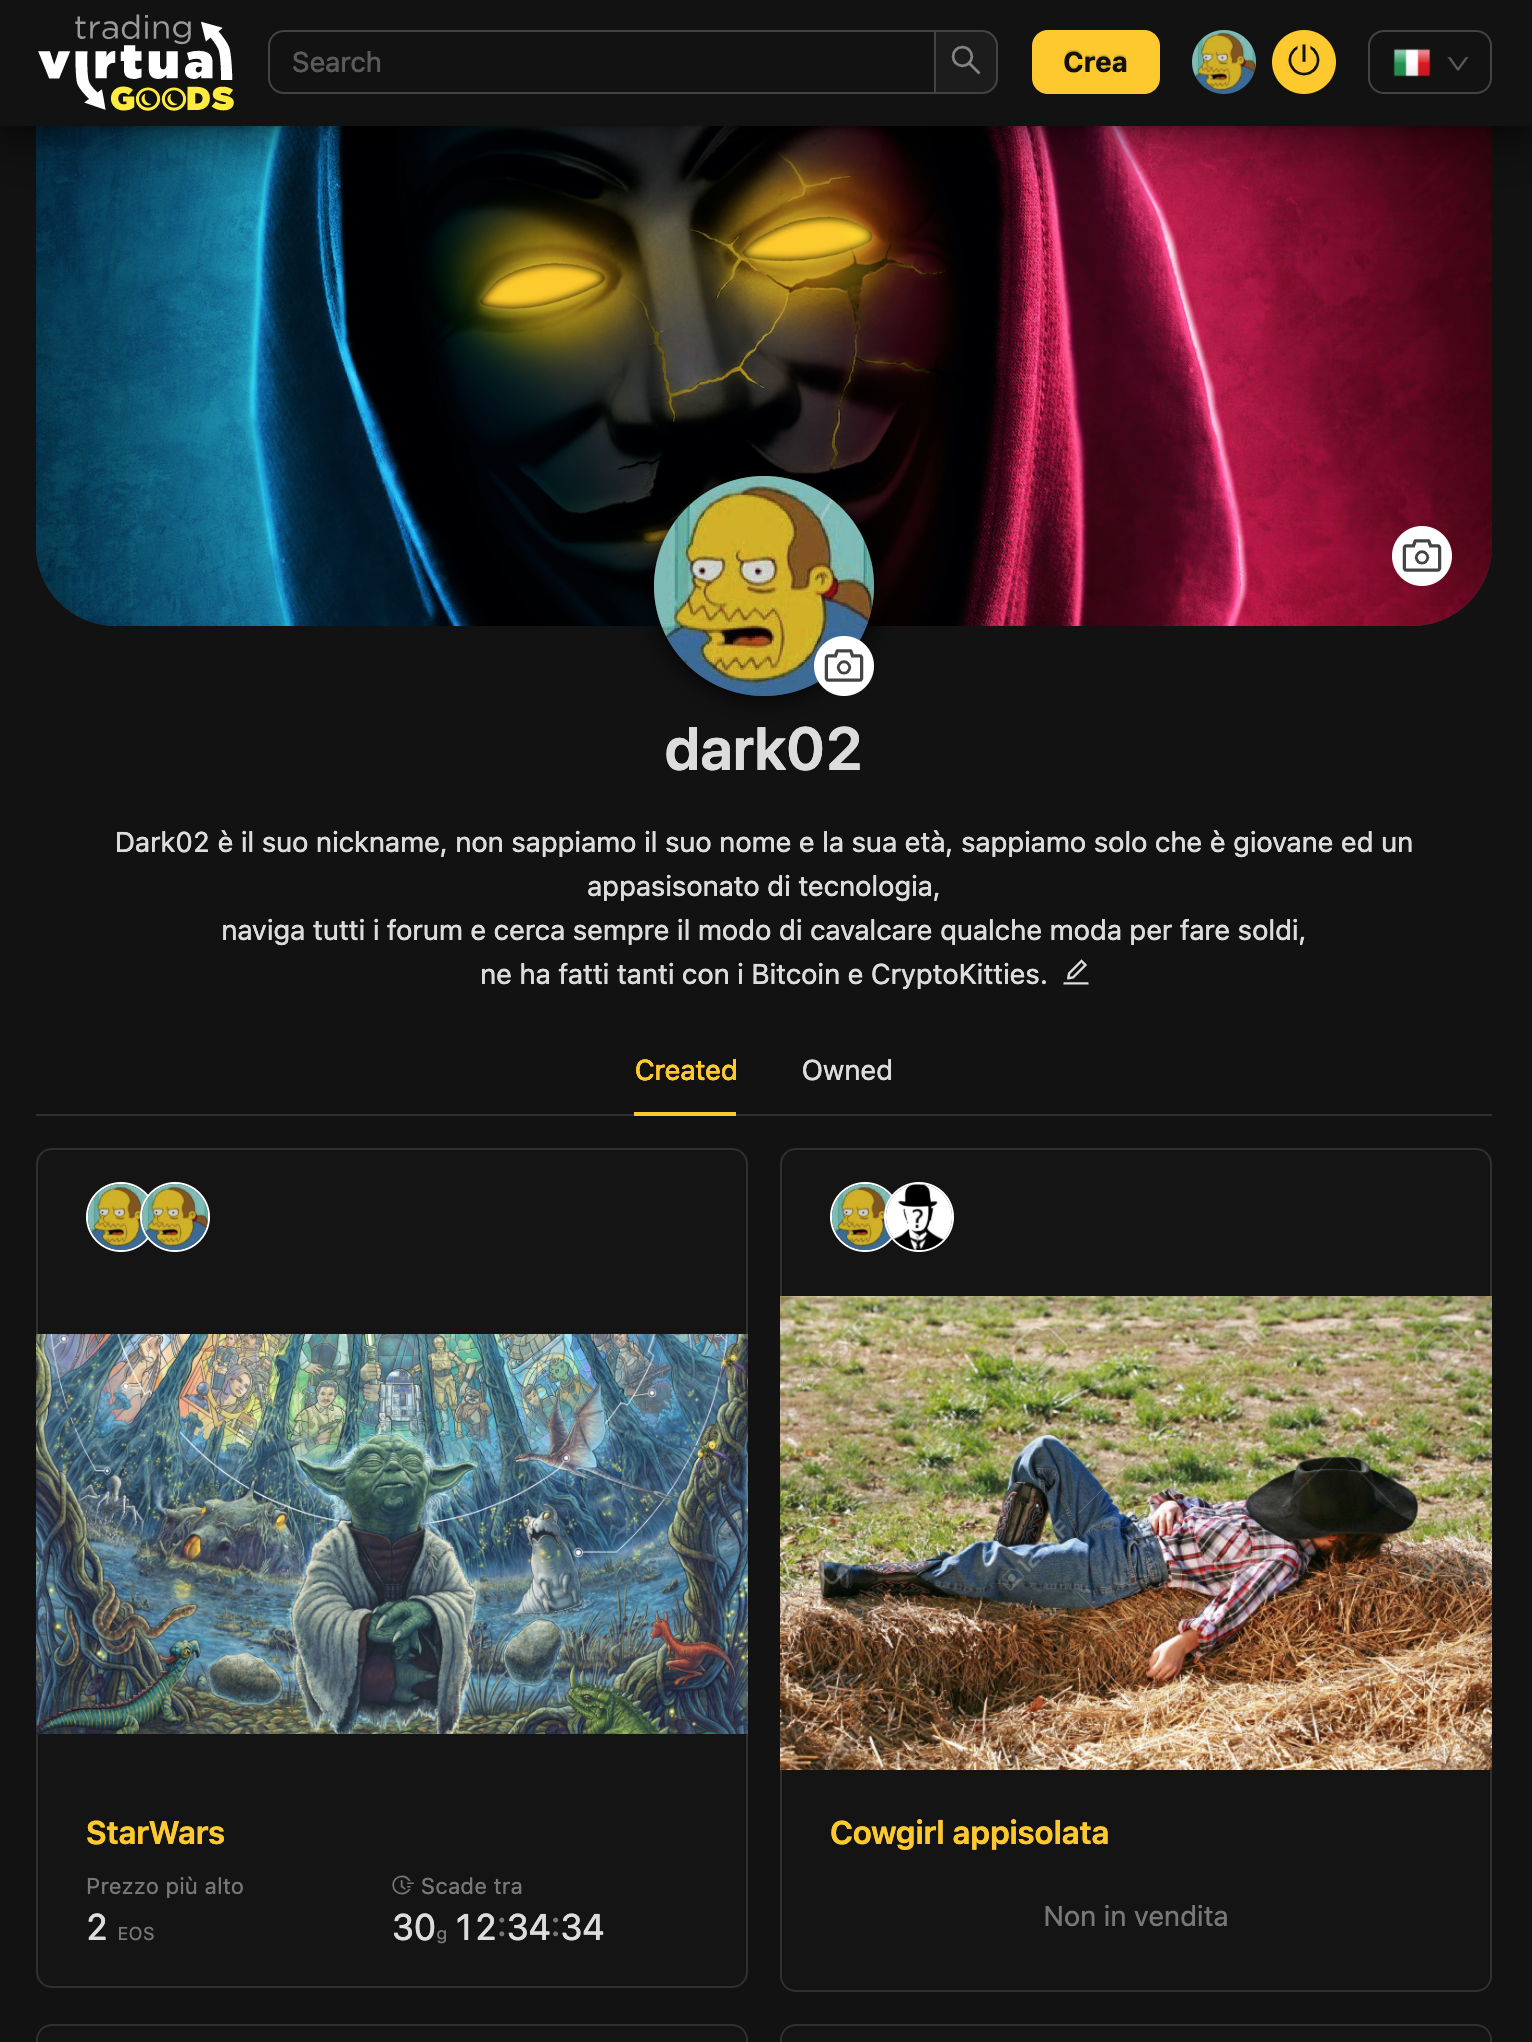
\includegraphics[width=\linewidth,keepaspectratio]{p-tablet-profile.jpg}
		\caption{Pagina profilo}
		\label{fig:pTabletProfile}
	\end{minipage}
\end{figure}

\begin{figure}[H]
	\centering
	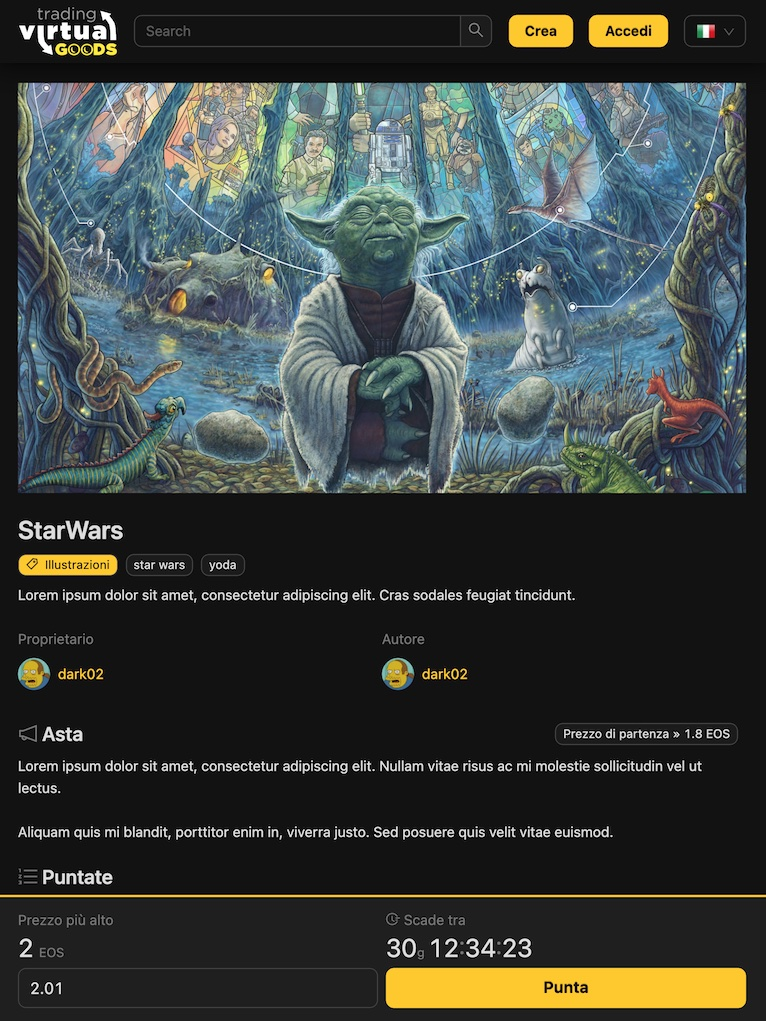
\includegraphics[width=0.75\textwidth,keepaspectratio]{p-tablet-auction.jpg}
	\caption{Pagina asta}
	\label{fig:pTabletAuction}
\end{figure}

\clearpage

\bigbreak
\noindent
\textbf{FullHD 1920x1080px}

\begin{figure}[H]
	\centering
	\includegraphics[width=\textwidth,keepaspectratio]{p-fullhd-auction.jpg}
	\caption{Pagina asta}
	\label{fig:pFullhdAuction}
\end{figure}

\clearpage

\bigbreak
\noindent
\textbf{Accesso/Registrazione}
\bigbreak
\noindent
Per quanto riguarda l'accesso e la registrazione al portale, abbiamo deciso di utilizzare un metodo "Google style": 
l'utente inserisce la sua email, il sistema controlla se è presente tra gli utenti registrati 
ed in caso positivo viene proposto il modulo di accesso con password.
In caso negativo viene proposto il modulo per la registrazione.

Questa scelta è data dal fatto che alcune tipologie di utente, soprattutto quelle di età adulta,
fanno confusione tra accesso e registrazione, non hanno ben chiaro il flusso tipico di un servizio web.
Può capitare che utenti registrati, per accedere al sito, tentano di registrarsi nuovamente.

Inoltre con questo metodo si alleggerisce l'interfaccia, inserendo un'unico pulsante "accedi" invece di due pulsanti "accedi" e "registrati".

\begin{figure}[H]
	\centering
	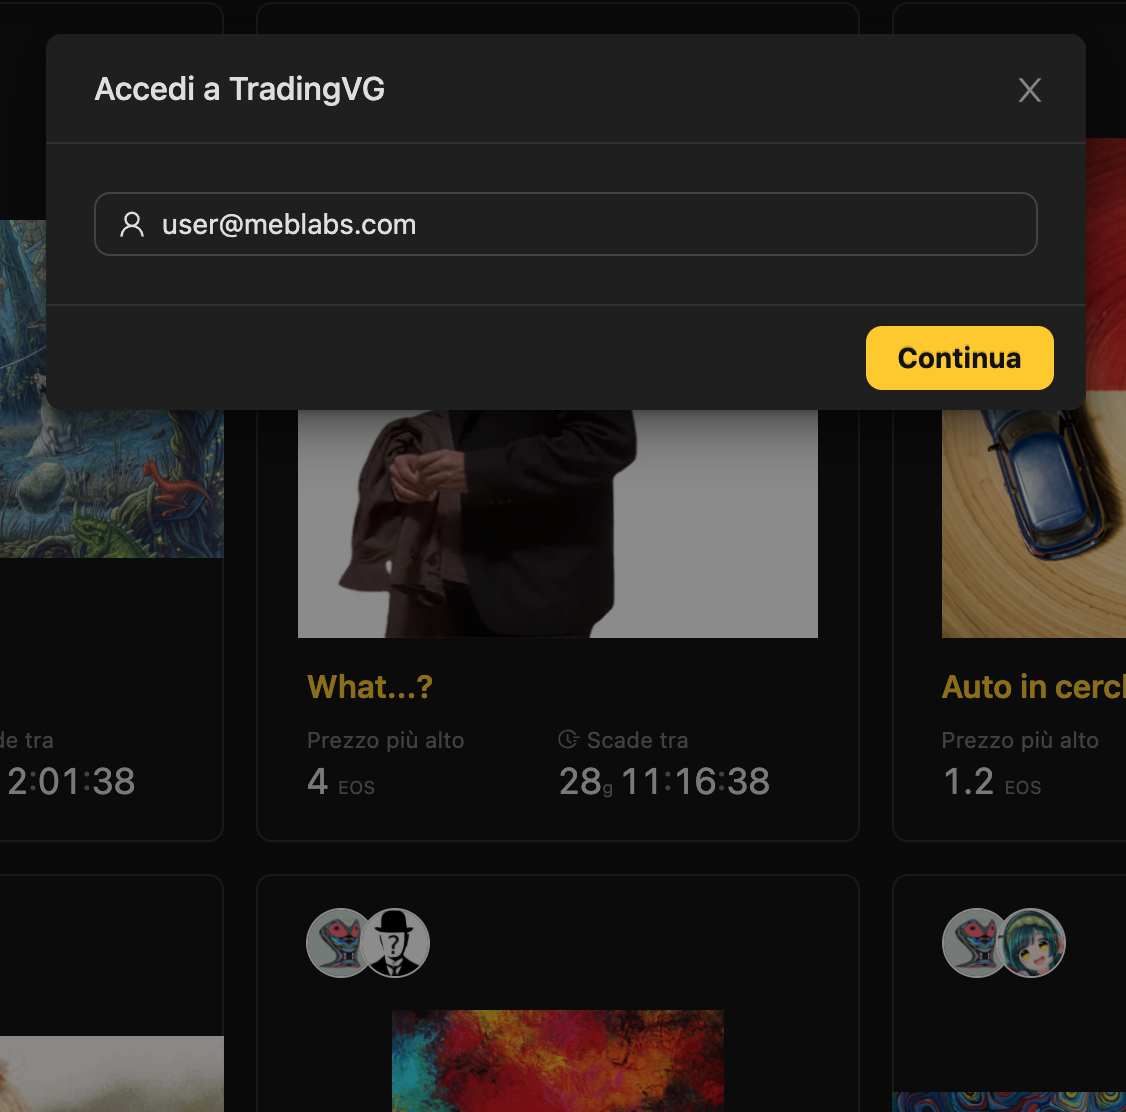
\includegraphics[width=0.85\textwidth,keepaspectratio]{p-check.jpg}
	\caption{Controllo email}
	\label{fig:pCheck}
\end{figure}

\begin{figure}[H]
	\centering
	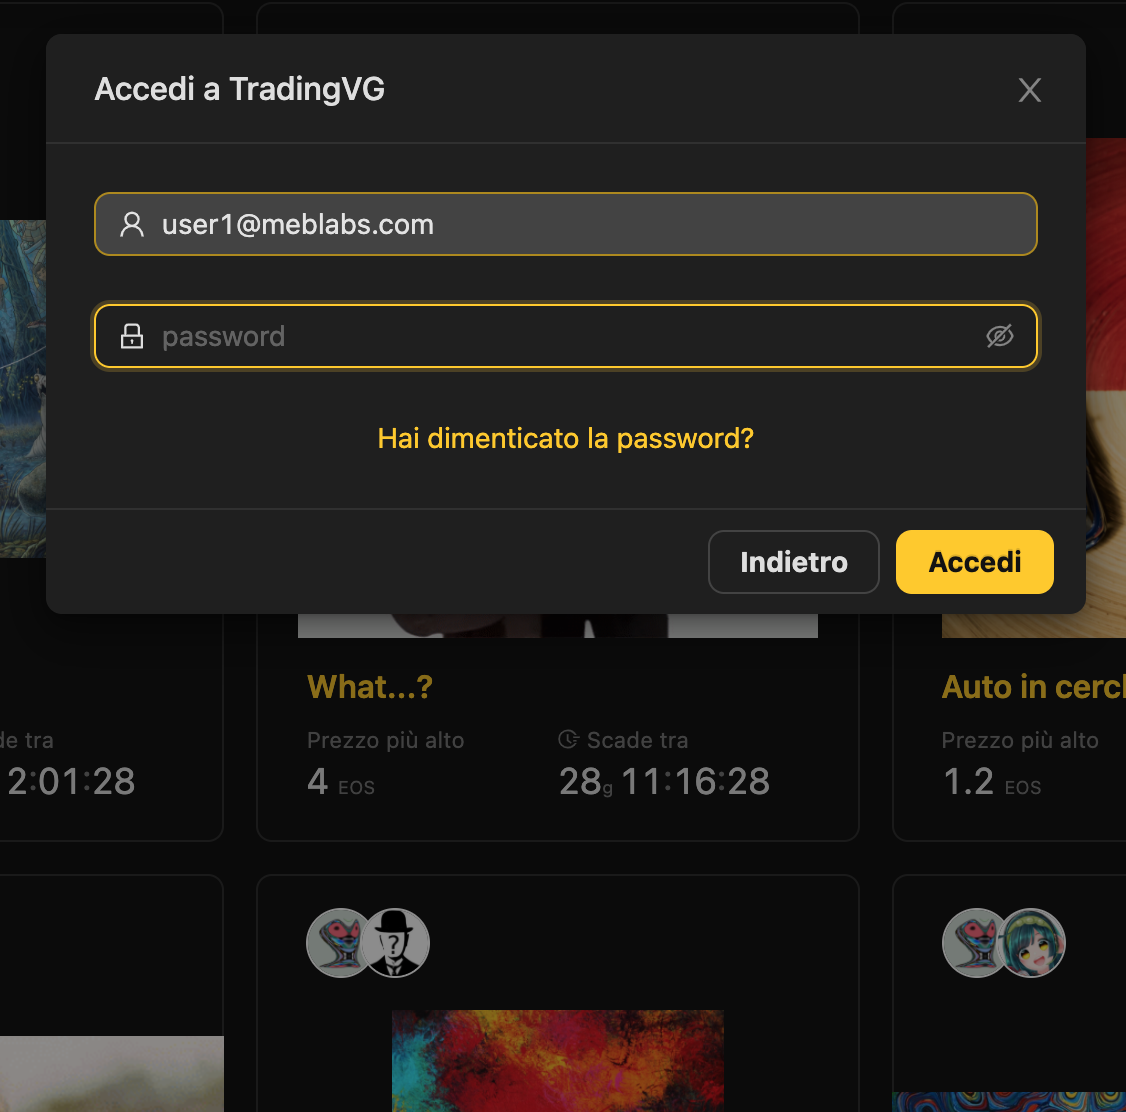
\includegraphics[width=0.85\textwidth,keepaspectratio]{p-login.jpg}
	\caption{Accesso con credenziali}
	\label{fig:pLogin}
\end{figure}

\begin{figure}[H]
	\centering
	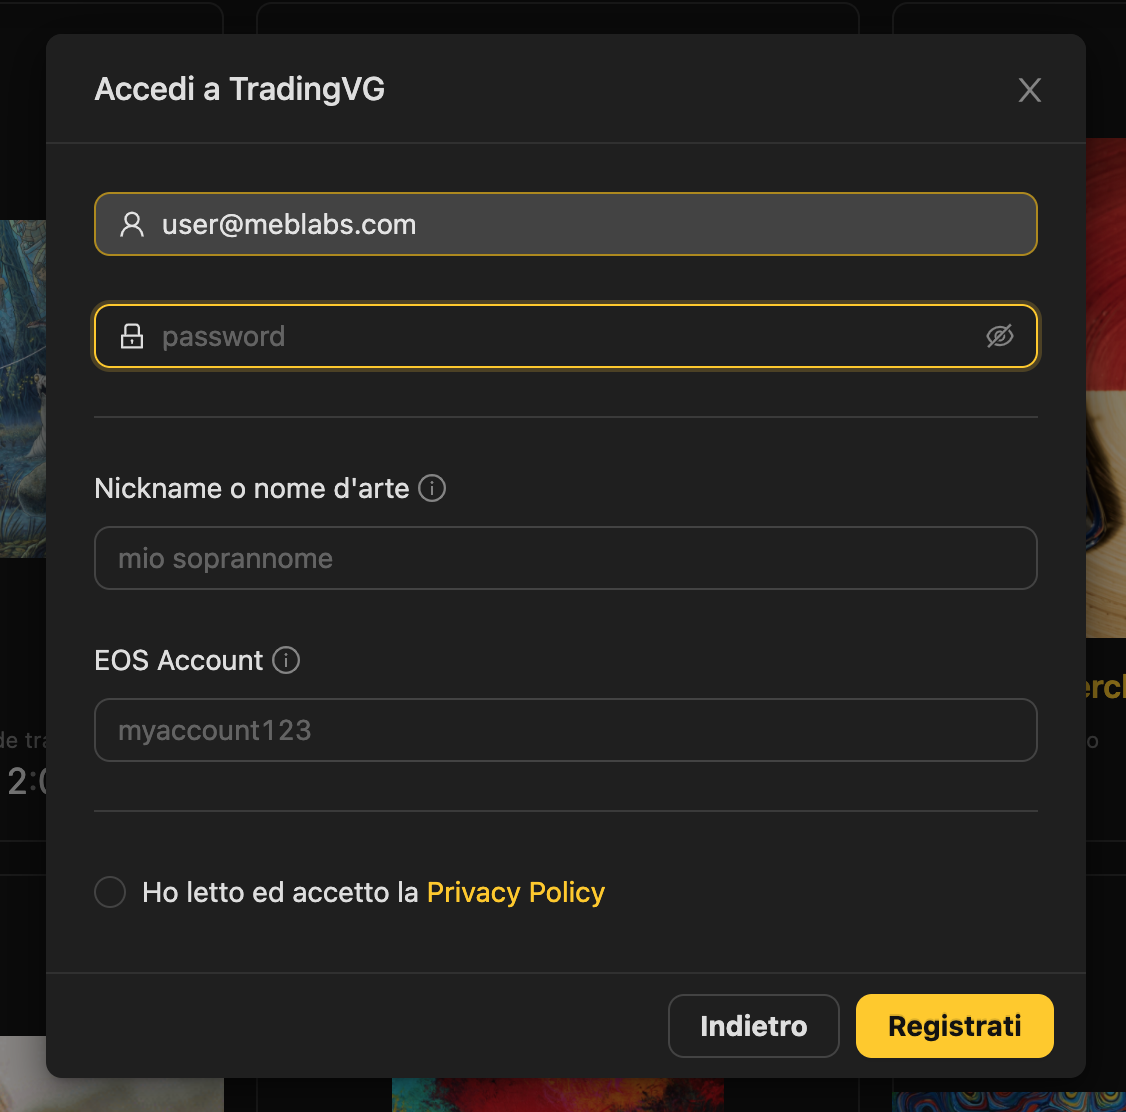
\includegraphics[width=0.85\textwidth,keepaspectratio]{p-register.jpg}
	\caption{Registrazione}
	\label{fig:pRegister}
\end{figure}
